\documentclass[11pt,
  letterpaper,
  openany,
  toc=bibliography,
  idxtotoc,
  bookmarks]{labbook}

\usepackage[utf8]{inputenc}
\usepackage[T1]{fontenc}
\usepackage[spanish]{babel}

\usepackage[margin=2.5cm]{geometry}
\usepackage{microtype}
\usepackage{graphicx}
\usepackage{amsmath,amssymb}
\usepackage{csquotes}
\usepackage{booktabs}
\usepackage{enumitem}
\usepackage{authblk}
\usepackage[spanish]{cleveref}
\usepackage[dvipsnames]{xcolor}
\usepackage{pgfplotstable}
\usepackage{siunitx}
\usepackage{subcaption}
\usepackage{multirow}

\pgfplotsset{compat=1.18}
\pgfkeys{/pgf/number format/1000 sep={\,}}

\AtBeginDocument{\decimalpoint}
\renewcommand{\arraystretch}{1.2}
\sisetup{group-digits=true,
  group-separator={\,},
  separate-uncertainty}

\usepackage[backend=biber,style=numeric]{biblatex}
\addbibresource{./references-pre-project.bib}

\usepackage{pdfbase}
\pdfinfo{
  /Title (Osciladores Acoplados - Bitácora de Laboratorio)
  /Author (Sebastián Rodríguez, Laura Torres, Julián Ávila)
  /Creator (LaTeX with labbook class)
}

\title{\textbf{Osciladores Acoplados} \\
Bitácora de Laboratorio}
\author{Sebastian Rodríguez \and Laura Torres \and Julian Avila}
\affil{Universidad Distrital Francisco José de Caldas}
\date{}

\begin{document}

\maketitle

\tableofcontents

\labday{Miércoles 23, Abril 2025}




\labday{Jueves 24, Abril 2025}

\experiment{Planteamiento Teórico}
Se desarrolla el fundamento teórico del problema de los tres péndulos
físicos acoplados por resortes. A partir del desplazamiento angular
de cada péndulo, \(\theta_i\), se establece el sistema planteado con
sus relaciones importantes, presentado en la \cref{fig:sistema-pendulos}.

\begin{figure}[htbp!]
  \centering
  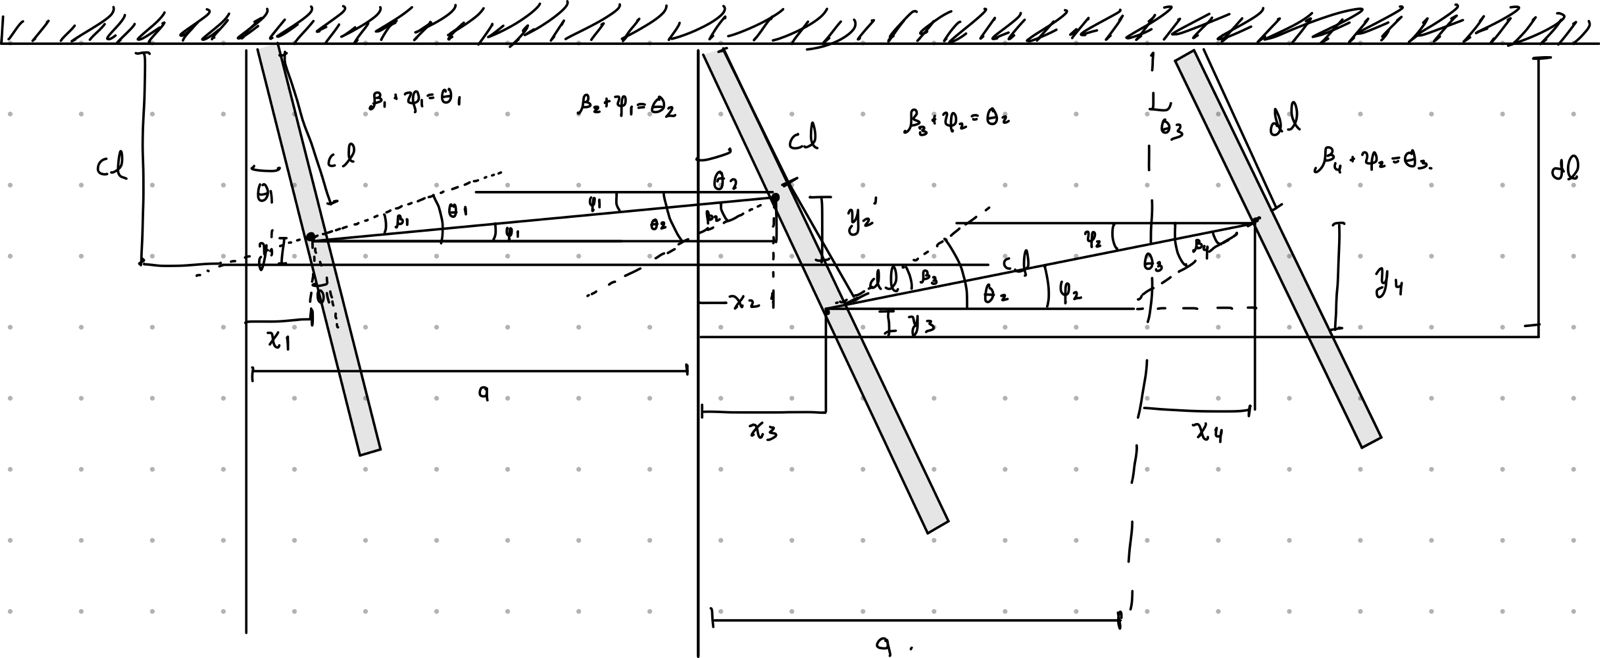
\includegraphics[width=0.8\linewidth]{Figures/IM1.jpeg}
  \caption{Sistema de tres péndulos físicos acoplados por resortes.}
  \label{fig:sistema-pendulos}
\end{figure}

Considerando el desplazamiento angular de cada péndulo, se determina
la suma de los torques que actúan sobre cada uno para derivar el
sistema de ecuaciones del movimiento.

La distancia \( a \) es la separación entre cada péndulo. \( cl \) es
la distancia a la cual se acoplan los péndulos 1 y 2 por medio del
resorte con constante \( k_1 \), mientras que \( dl \) es la distancia
de acople entre 2 y 3 por medio del resorte con constante \( k_2 \).
Los \(y_{\text{cm}_i}\) corresponden a la distancia desde el punto de
giro al centro de masa. De esta forma, el torque restaurador
gravitacional está relacionado con \(m_i g y_{\text{cm}_i} \sin{\theta_i}\).

Para las interacciones generadas por los resortes, se asume que
obedecen a la ley de Hooke lineal y que actúan a lo largo de una
línea de acción horizontal. De esta forma, se aplicará una
aproximación lineal a todos los términos angulares no lineales.

La sumatoria de torques para cada péndulo genera el siguiente
sistema de ecuaciones diferenciales:

\begin{equation}
  \begin{aligned}
    \ddot{\theta}_1 =\; &
    -\theta_1 \left[ \frac{k_1 (cl)^2 + y_{\text{cm}_1} m_1 g}{I_1} \right]
    + \theta_2 \left( \frac{k_1 (cl)^2}{I_1} \right) \\[0.5em]
    \ddot{\theta}_2 =\; &
    \theta_1 \left( \frac{k_1 (cl)^2}{I_2} \right)
    - \theta_2 \left[ \frac{k_1 (cl)^2 + k_2 (dl)^2 + y_{\text{cm}_2} m_2 g}{I_2} \right]
    + \theta_3 \left( \frac{k_2 (dl)^2}{I_2} \right) \\[0.5em]
    \ddot{\theta}_3 =\; &
    \theta_2 \left( \frac{k_2 (dl)^2}{I_3} \right)
    - \theta_3 \left[ \frac{k_2 (dl)^2 + y_{\text{cm}_3} m_3 g}{I_3} \right]
  \end{aligned}
\end{equation}

\experiment{Características Experimentales}
Adicionalmente, se establecen las características clave del montaje
experimental, buscando cumplir con las siguientes condiciones:

\begin{itemize}
  \item Usar barras masivas, de modo que, en comparación con
    constantes elásticas bajas de los resortes, se obtengan series
    de tiempo extensas. Esto es importante, ya que en el caso real
    se tiene rozamiento con el aire y en las zonas de contacto
    (rodamientos).
  \item Utilizar resortes que se aproximen al muelle ideal,
    manteniendo su linealidad y capacidad de operar bajo fuerzas
    compresivas y extensivas. Se buscarán constantes elásticas
    suficientemente pequeñas para permitir oscilaciones extensas y
    claras.
  \item Obtener barras ``ideales'', donde los puntos de contacto
    estén centrados y equidistantes en las tres barras.
\end{itemize}

Para lograr esto, se buscarán barras muy masivas, fabricadas con
un material de alta densidad, como un metal, descartando el aluminio
en primera aproximación debido a su baja densidad. Para la toma de
datos, se utilizarán sensores rotacionales angulares CASSY. Se
acoplará un sensor a cada péndulo/barra, aprovechando que cada sensor
está montado en un rodamiento que permite mayor libertad de
movimiento y cuenta con un soporte para colgar los objetos que rotan.

\begin{figure}[htbp!]
  \centering
  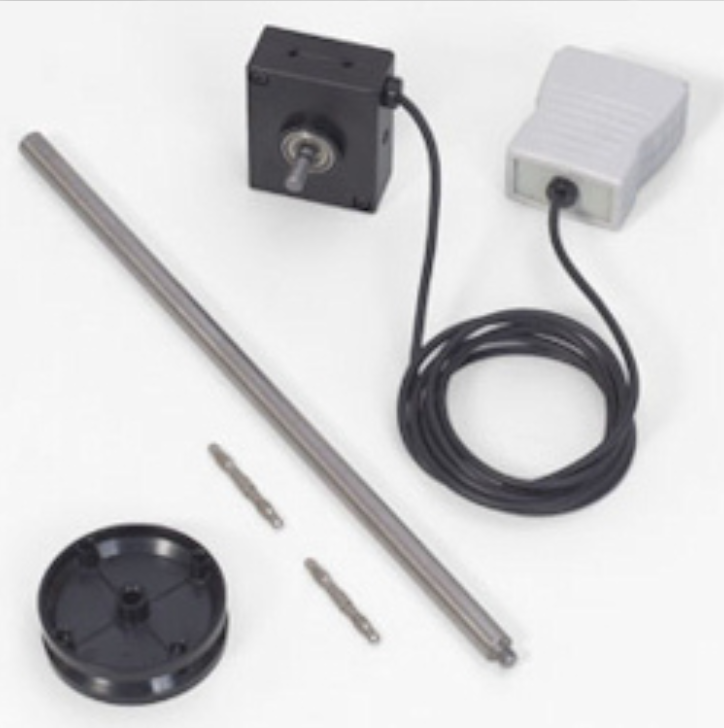
\includegraphics[width=0.5\linewidth]{Figures/IM2.png}
  \caption{Sensor CASSY de movimiento angular.}
  \label{fig:cassy}
\end{figure}


\labday{Miércoles 30, Abril 2025}

\experiment{Construcción del Montaje}

Para la construcción de los péndulos físicos, se utilizaron barras
metálicas obtenidas en el taller de máquinas y herramientas de la
sede Macarena, las cuales cumplían con el requisito previamente
planteado de emplear un material con alta densidad.
Del mismo modo, se avanzó en la preparación del sistema de medición
de ángulos mediante el sensor Cassy, revisando su funcionamiento,
calibración y evaluando la forma de integrarlo al sistema.
Para finalizar, se llevó a cabo la medición de la constante
elástica de los resortes inicialmente seleccionados para la
práctica. Estos resortes fueron adquiridos en una fábrica
especializada con el fin de garantizar constantes elásticas
nominales similares y condiciones físicas consistentes.

\subexperiment{Construcción de los péndulos}
En el taller se identificó una varilla metálica de sección
adecuada. Esta varilla presentaba la rigidez necesaria para
nuestro experimento, por lo que se decidió utilizarla.
A partir de ella, se cortaron las barras con las longitudes
especificadas para el sistema (\(l\) para el central y \(l/2\)
para los laterales). Posteriormente, se pulieron los bordes
para evitar imperfecciones o filos peligrosos, y se perforaron
los orificios necesarios para su montaje.
En el caso de las barras de longitud \(l/2 = \qty{28.0(1)}{\centi\metre}\),
los orificios se realizaron a una distancia de \qty{4.6(1)}{\centi\metre}
desde cada extremo.

Adicionalmente, se midieron las masas de las barras y se determinó
la posición de sus respectivos centros de masa,
medidos desde el punto de pivote. Los resultados se resumen en la
\cref{tab:bars-dat}.

\pgfplotstableread[col sep=comma, header=true]{
	i, y_cm_i, m_i
	1, 14.2, 0600.8
	2, 28.0, 1216.3
	3, 14.0, 0601.8
}\mydata

\begin{table}[htbp!]
	\centering
	\pgfplotstabletypeset[
	col sep=comma,
	zerofill,
	columns/i/.style={
		string type,
		column type={c},
		column name={\(i\)},
	},
	columns/y_cm_i/.style={
		column name={\(y_{\text{cm}_i} [\si{\centi\metre}]\)},
		precision=1,
		fixed,
		fixed zerofill,
	},
	columns/m_i/.style={
		column type={c},
		column name={\(m_i [\si{\gram}]\)},
		dec sep align,
		precision=1,
		fixed,
		fixed zerofill,
	},
	every head row/.style={
		before row=\toprule,
		after row=\midrule,
	},
	every last row/.style={
		after row=\bottomrule,
	}
	]\mydata
	\caption{Parámetros físicos de las barras empleadas en el montaje.
		La incertidumbre para la posición del centro de masa (\(y_{\text{cm}_i}\))
		es de \qty{0.1}{\centi\metre} y para la masa (\(m_i\)) es de
	\qty{0.1}{\gram}.}
	\label{tab:bars-dat}
\end{table}

\begin{figure}[htbp!]
	\centering
	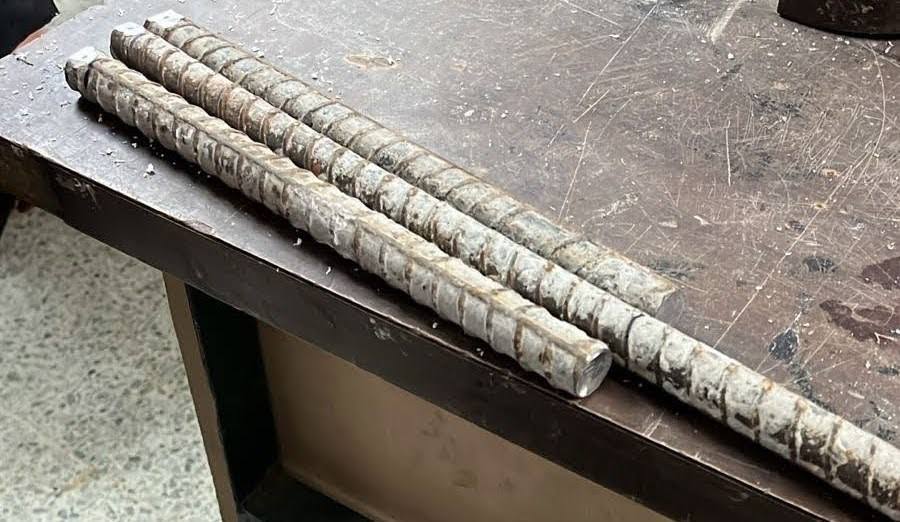
\includegraphics[width=0.7\linewidth]{./Figures/metal-bars.jpeg}
	\caption{Barras metálicas preparadas para el montaje de los péndulos.}
	\label{fig:metal-bars}
\end{figure}

\subexperiment{Preparación del Dispositivo \emph{Cassy}}
Se realizó una revisión inicial del sistema de medición Cassy.
Esta observación permitió definir una estrategia preliminar para
su integración en el sistema, con el fin de registrar los
ángulos de oscilación. Se empleará alambre dulce para fijar las
barras a la rueda giratoria de cada sensor, utilizando los
orificios correspondientes en ambas partes.

\subexperiment{Medición de la constante elástica}
Se llevó a cabo la medición de la constante elástica de los
resortes que se planea utilizar en el experimento. Para esto,
se empleó el montaje experimental convencional de aplicar masas
conocidas a cada resorte, medir su elongación y, mediante una
regresión lineal de desplazamiento en función de la masa soportada,
estimar su constante de elasticidad.

Se utilizaron masas en un rango de \qty{50}{\gram} a \qty{80}{\gram}.
Para dos resortes representativos, se obtuvieron constantes de
elasticidad de \(k_1 = \qty{3.04(4)}{\N\per\m}\) y
\(k_2 = \qty{3.32(6)}{\N\per\m}\). Los valores de desplazamiento
según la masa aplicada se presentan en la \cref{fig:springs-plot}.

\begin{figure}[htbp!]
	\centering
	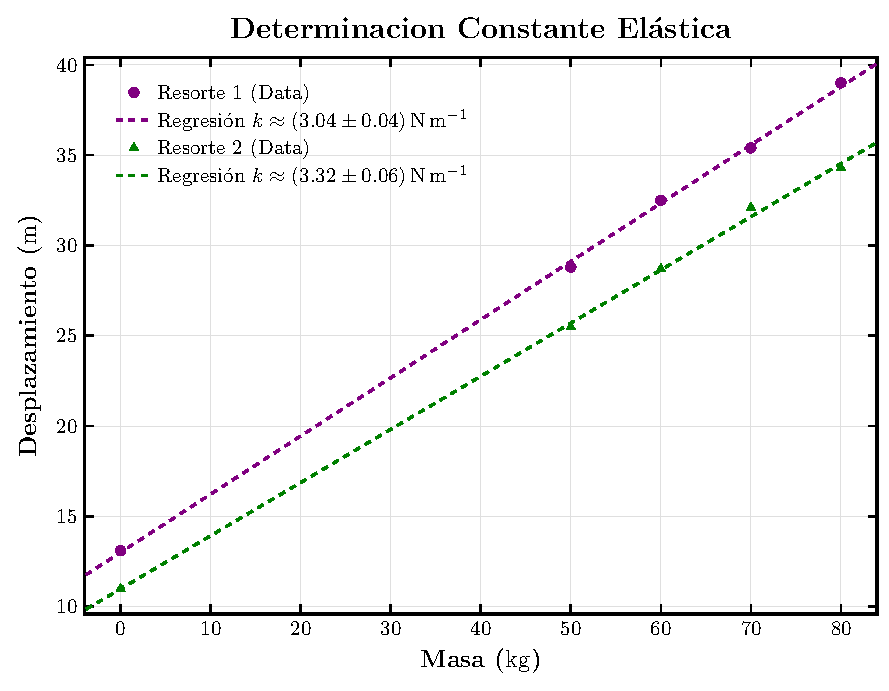
\includegraphics[width=0.6\linewidth]{./Figures/springs-plot.pdf}
	\caption{Determinación de la constante elástica de los resortes.}
	\label{fig:springs-plot}
\end{figure}


\labday{Miércoles 07, Mayo 2025}

\experiment{Toma de Datos Experimentales}

Para la adquisición de datos, se ensambló completamente el sistema de
tres péndulos físicos acoplados. Se instaló un sensor rotacional
\emph{Cassy} en el soporte de cada péndulo, alineado coaxialmente con su
eje de giro. Esta disposición, visible en la \cref{fig:set-up},
permitió registrar el desplazamiento angular \(\theta_i(t)\) de cada
barra de forma independiente. Los resortes de acoplamiento se fijaron
a las barras según las especificaciones del diseño experimental,
estableciendo así la interacción mecánica entre los péndulos.

Una vez configurado el montaje, se realizaron mediciones para cinco
distintas configuraciones de acoplamiento del sistema. Estas
configuraciones, que varían los puntos de anclaje de los resortes
entre los péndulos, se ilustran esquemáticamente en la
\cref{fig:configs}, junto con la codificación utilizada para
identificarlas. Para cada una de estas cinco configuraciones,
el sistema se observó bajo tres condiciones de excitación inicial
(desplazamiento angular inicial):
\begin{itemize}
	\item Desplazamiento de un solo péndulo lateral (i.e. péndulo 1),
		codificado como (100).
	\item Desplazamiento del péndulo central (péndulo 2), codificado
		como (010).
	\item Desplazamiento simultáneo y simétrico (o antisimétrico,
		según el caso) de los dos péndulos laterales (péndulos 1 y 3),
		codificado como (101).
\end{itemize}
Los datos de la evolución temporal del ángulo de cada péndulo para
cada ensayo fueron registrados automáticamente por el sistema \emph{Cassy}
y almacenados digitalmente para su posterior análisis. Se procuró
que cada registro tuviera una duración aproximada de
\qty{30}{\second} para capturar múltiples oscilaciones.

\begin{figure}[htbp!]
	\centering
	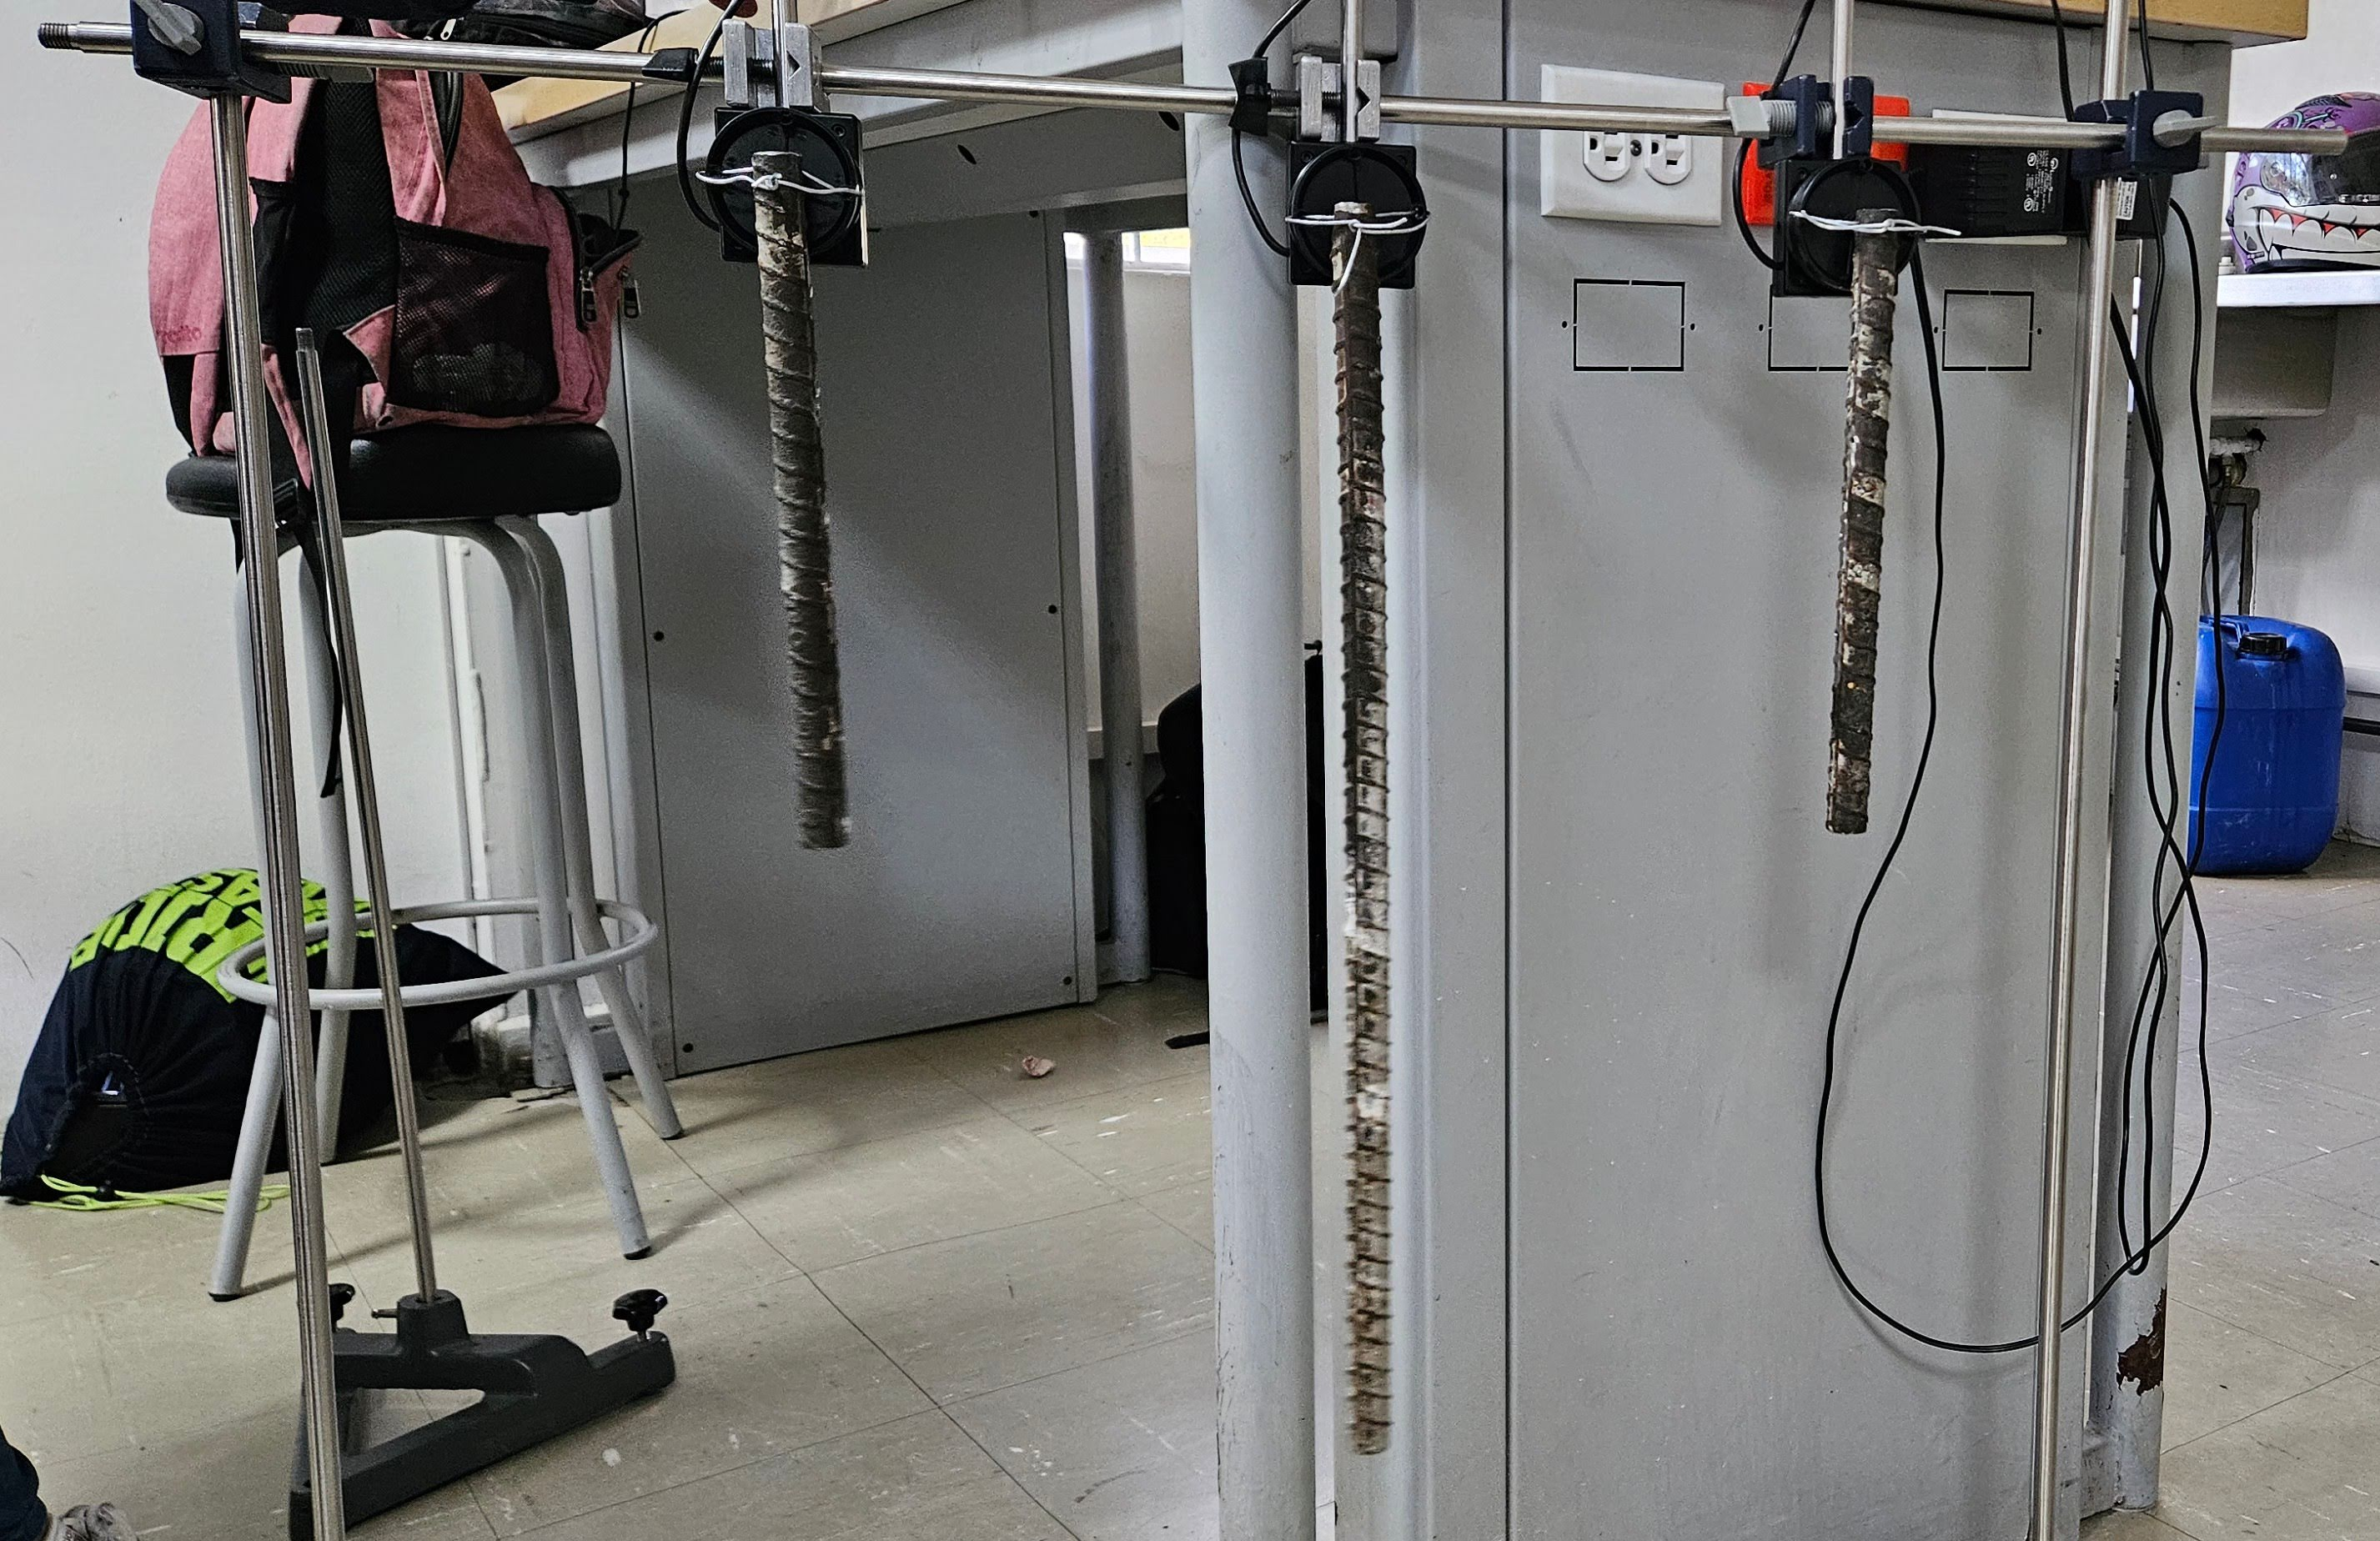
\includegraphics[width=0.6\linewidth]{./Figures/set-up.jpeg}
	\caption{Montaje experimental completo con los tres péndulos
		acoplados y los sensores rotacionales \emph{Cassy} posicionados para
	medir el ángulo de cada péndulo.}
	\label{fig:set-up}
\end{figure}

\begin{figure}[htbp!]
	\centering
	\begin{subfigure}[b]{0.3\textwidth}
		\centering
		\scalebox{-1}[1]{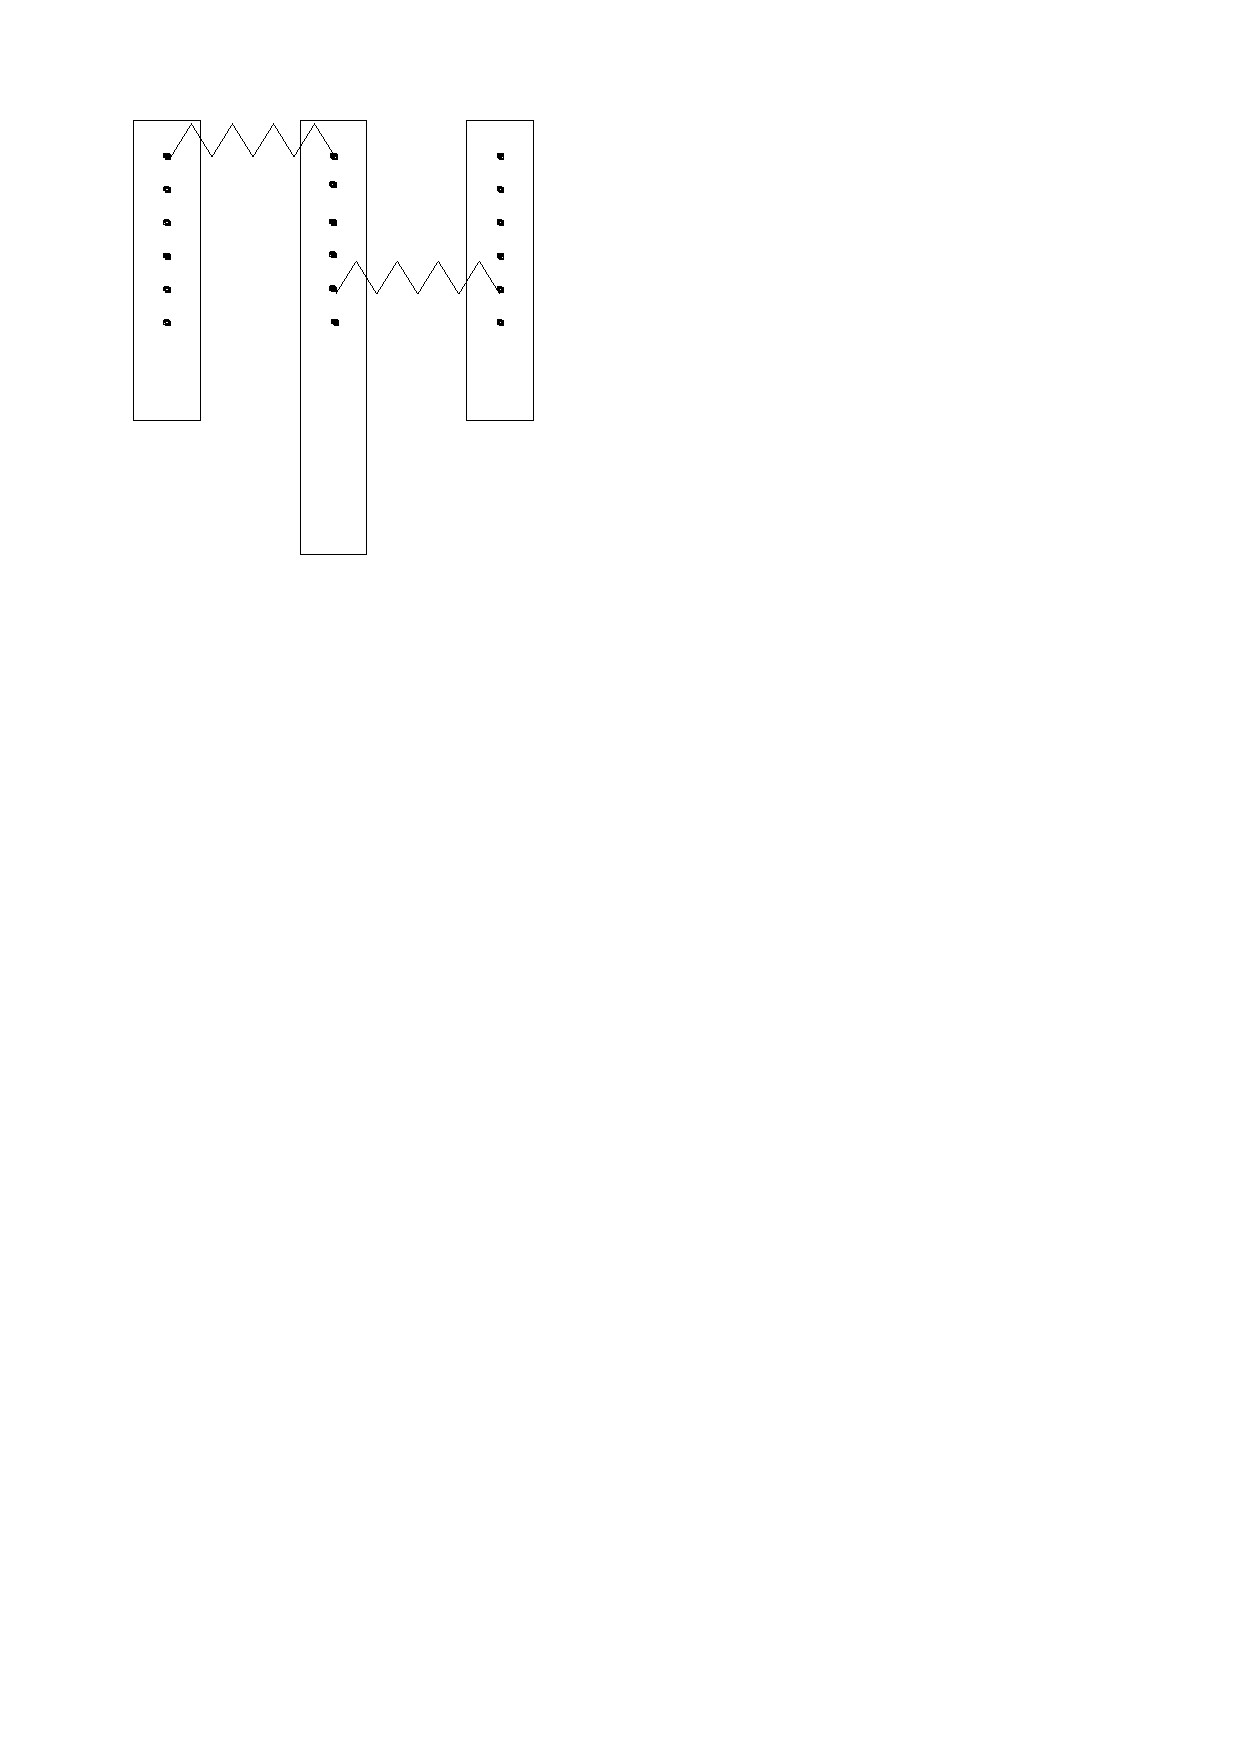
\includegraphics[width=\linewidth]{./Figures/15.pdf}}
		\caption{Configuración 5-1}
		\label{fig:conf-1-5}
	\end{subfigure}
	\hfill
	\begin{subfigure}[b]{0.3\textwidth}
		\centering
		\scalebox{-1}[1]{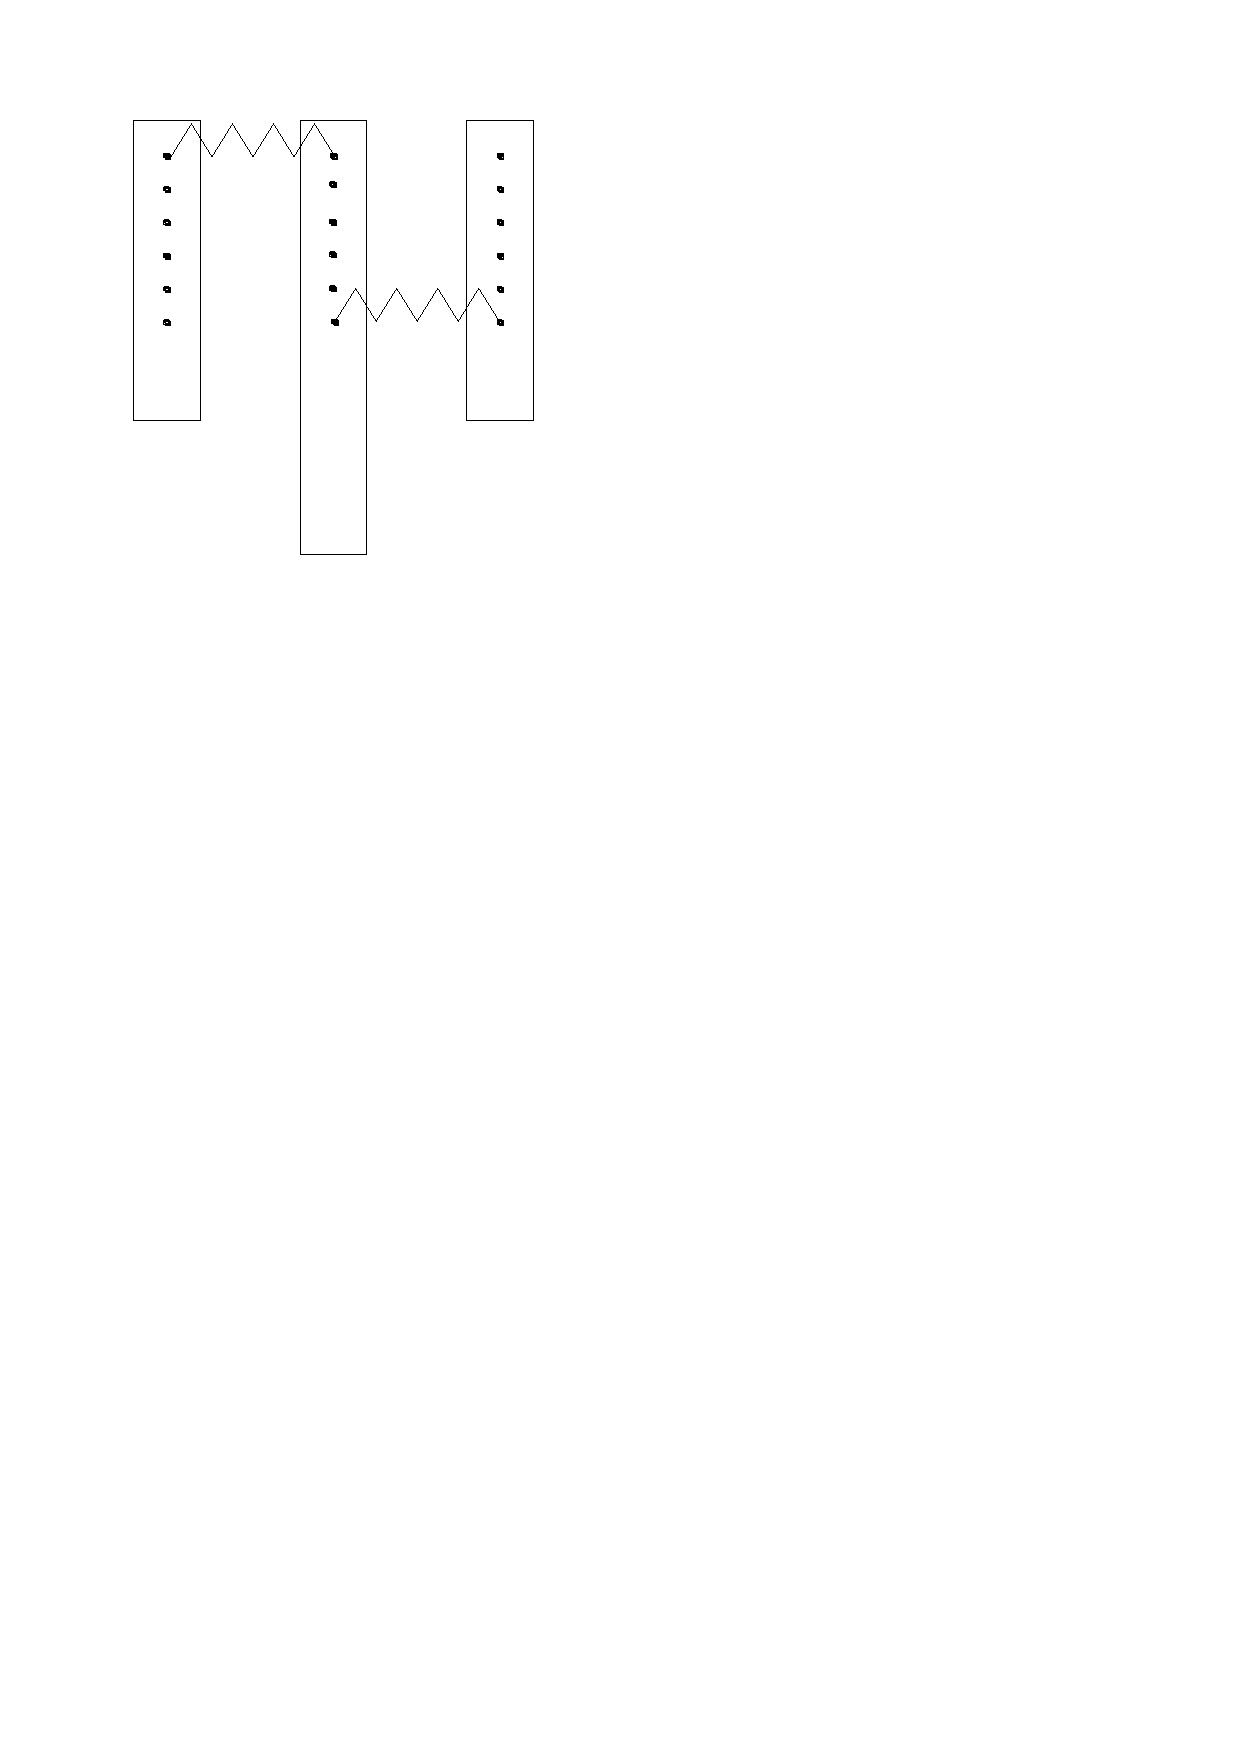
\includegraphics[width=\linewidth]{./Figures/16.pdf}}
		\caption{Configuración 6-1}
		\label{fig:conf-1-6}
	\end{subfigure}
	\hfill
	\begin{subfigure}[b]{0.3\textwidth}
		\centering
		\scalebox{-1}[1]{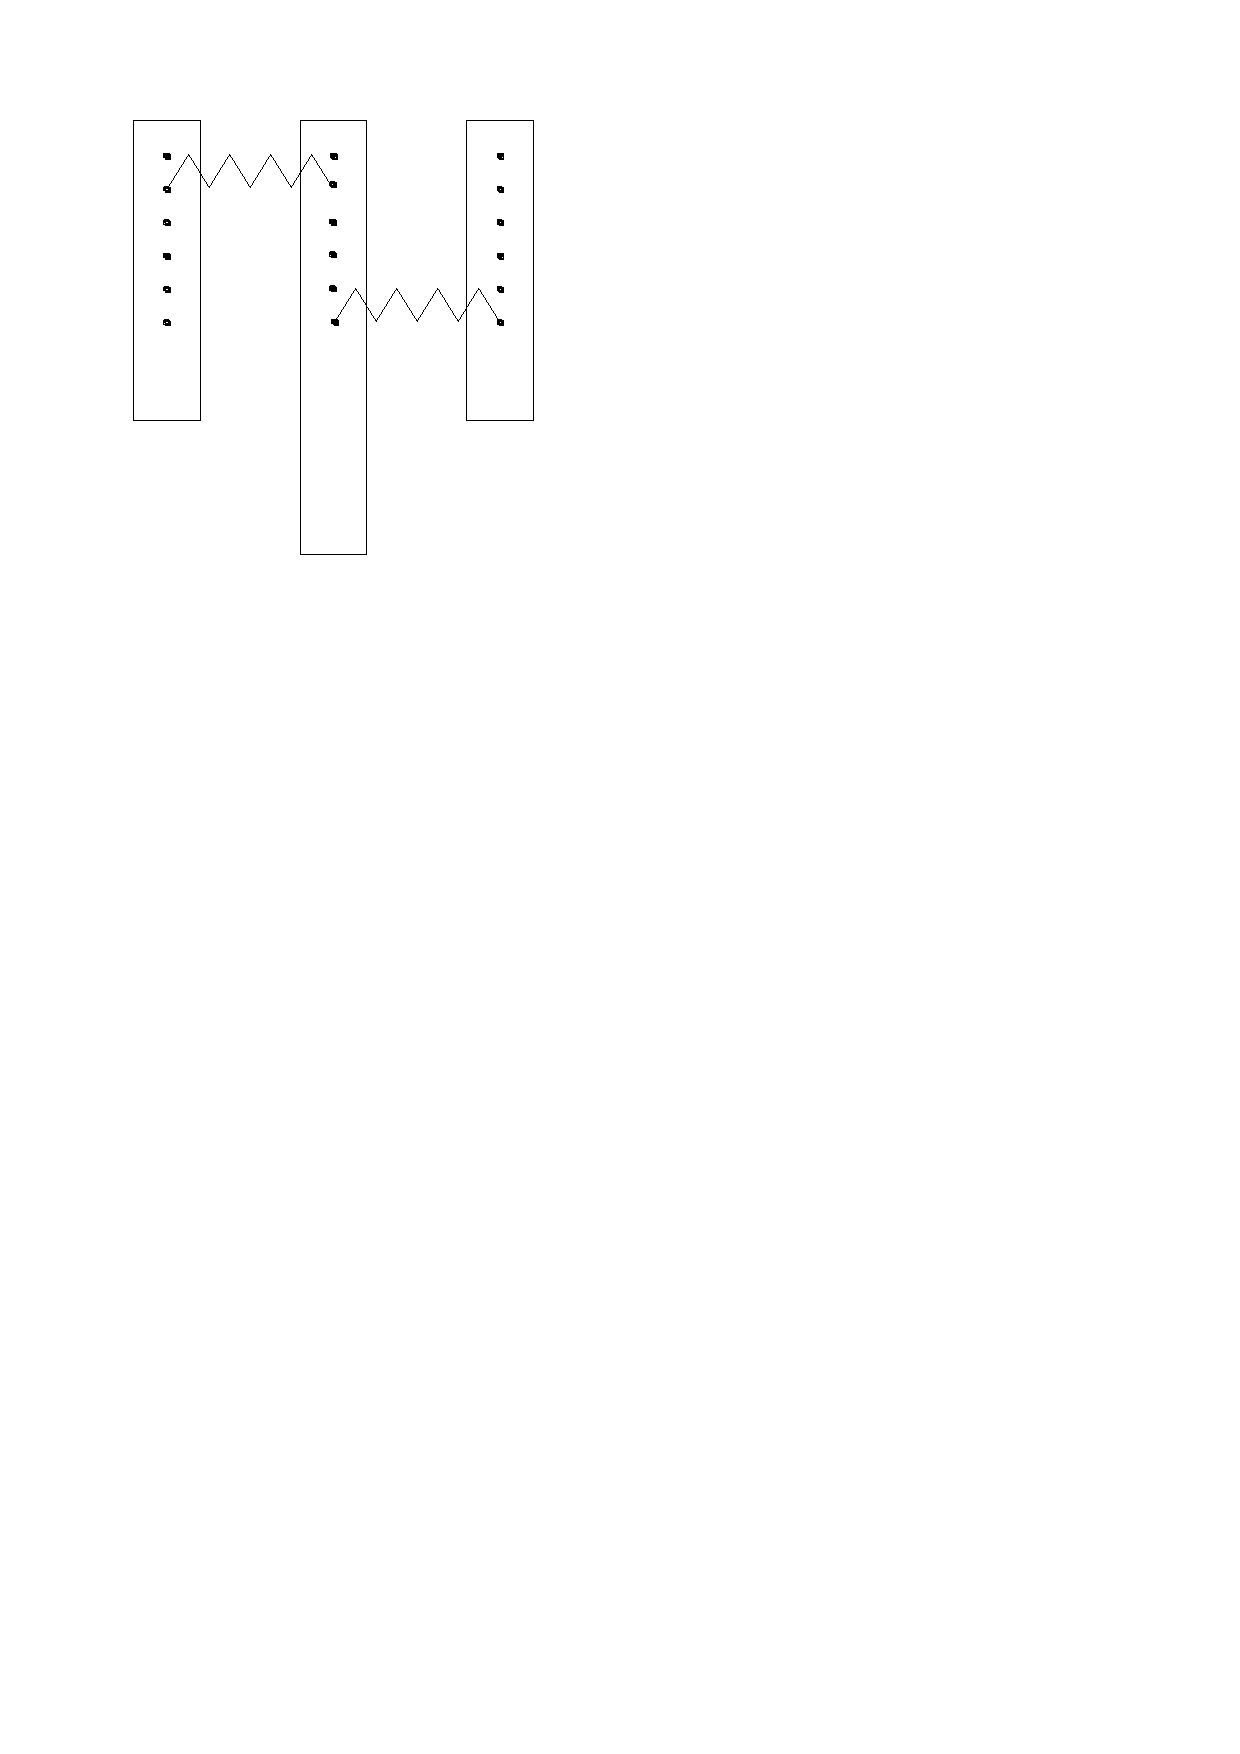
\includegraphics[width=\linewidth]{./Figures/26.pdf}}
		\caption{Configuración 6-2}
		\label{fig:conf-2-6}
	\end{subfigure}

	\vspace{0.5cm}

	\begin{subfigure}[b]{0.3\textwidth}
		\centering
		\scalebox{-1}[1]{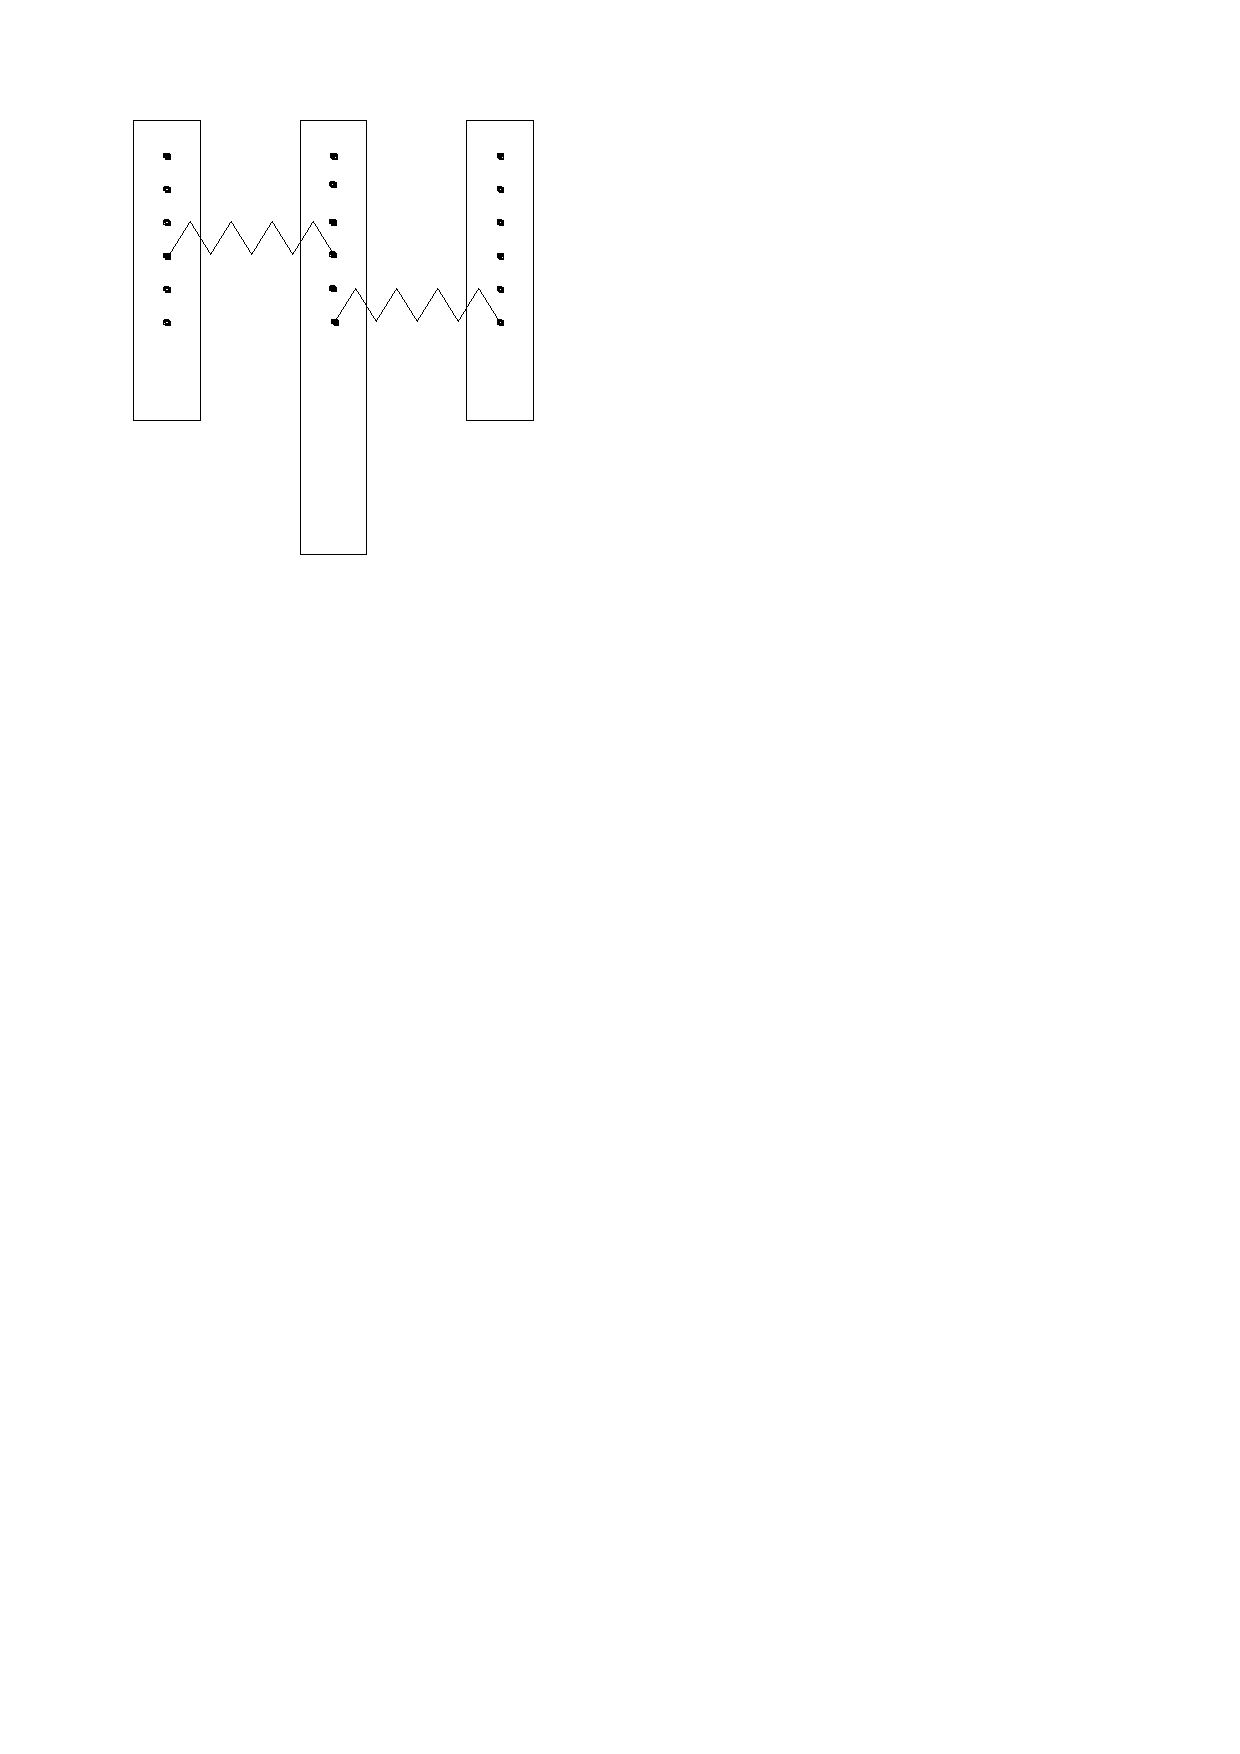
\includegraphics[width=\linewidth]{./Figures/46.pdf}}
		\caption{Configuración 6-4}
		\label{fig:conf-4-6}
	\end{subfigure}
	\hspace{0.1\textwidth}
	\begin{subfigure}[b]{0.3\textwidth}
		\centering
		\scalebox{-1}[1]{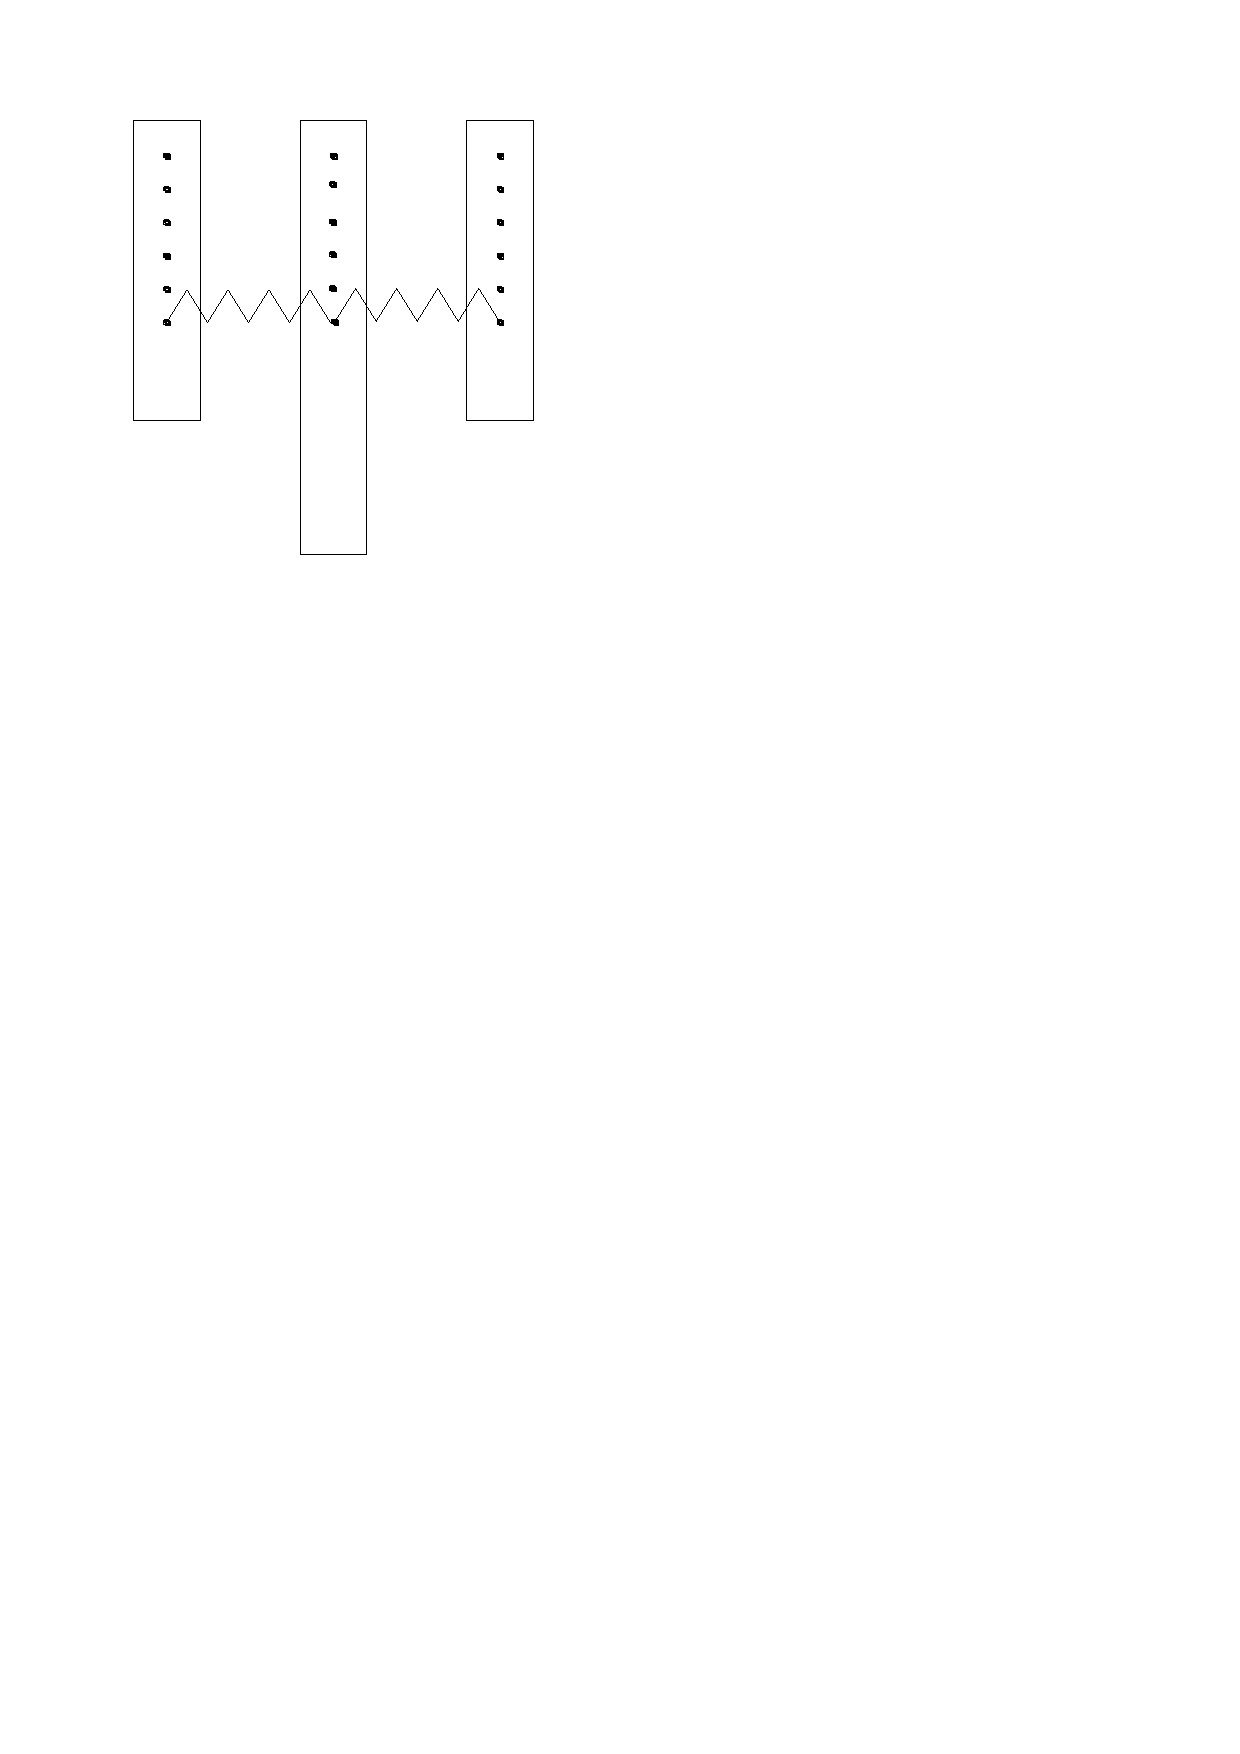
\includegraphics[width=\linewidth]{./Figures/66.pdf}}
		\caption{Configuración 6-6}
		\label{fig:conf-6-6}
	\end{subfigure}

	\caption{Representación esquemática de las cinco configuraciones de
		acoplamiento de resortes estudiadas. La nomenclatura 'X-Y' en cada
		subfigura (e.g. 5-1) denota los puntos de anclaje de los resortes
	en orificios específicos de los péndulos adyacentes.}
	\label{fig:configs}
\end{figure}


\labday{Resultados y Análisis}

\pgfplotstableread[col sep=comma, header=true]{
  i, y_cm_i, m_i
  1, 14.2, 600.8
  2, 28.0, 1216.3
  3, 14.0, 601.8
}\mydata

\pgfplotstableread[col sep=comma, header=true]{
  config, mode, freq1, freq2, freq3
  \multirow{3}{*}{5-1}, 100, 1.2715, 0.8408, 0.0205
  , 010, 0.8308, 0.8308, 0.8308
  , 101, 1.2771, 0.8375, 1.1934
  \multirow{3}{*}{6-1}, 100, 1.3147, 0.8383, 1.2003
  , 010, 0.8415, 0.8415, 0.8415
  , 101, 1.3144, 0.8348, 1.1901
  \multirow{3}{*}{6-2}, 100, 1.3303, 0.8455, 1.2288
  , 010, 0.8378, 0.8378, 0.8378
  , 101, 1.3189, 0.8402, 1.2114
  \multirow{3}{*}{6-4}, 100, 1.3263, 0.8547, 1.3263
  , 010, 0.8498, 0.8498, 0.8498
  , 101, 1.3250, 0.8505, 1.2713
  \multirow{3}{*}{6-6}, 100, 1.3144, 0.8552, 1.3303
  , 010, 0.8519, 0.8519, 0.8519
  , 101, 1.3147, 0.8574, 1.3474
}\datafreq

\pgfplotstableread[col sep=comma, header=true]{
  config, f1, f2, f3
  5-1, 1.1669, 0.8305, 1.2647
  6-1, 1.1669, 0.8343, 1.3120
  6-2, 1.1815, 0.8366, 1.3120
  6-4, 1.2394, 0.8437, 1.3122
  6-6, 1.3100, 0.8513, 1.3356
}\theoric

\pgfplotstableread[col sep=comma, header=true]{
  config, fe, ft, err
  \multirow{3}{*}{5-1}, 0.8308, 0.8305, 0.0361
  , 1.1934, 1.1669, 2.2205
  , 1.2771, 1.2647, 0.9709
  \multirow{3}{*}{6-1}, 0.8415, 0.8343, 0.8556
  , 1.1901, 1.1669, 1.9494
  , 1.3144, 1.3120, 0.1826
  \multirow{3}{*}{6-2}, 0.8378, 0.8366, 0.1432
  , 1.2114, 1.1815, 2.4682
  , 1.3189, 1.3120, 0.5232
  \multirow{3}{*}{6-4}, 0.8498, 0.8437, 0.7178
  , 1.2713, 1.2394, 2.5092
  , 1.3250, 1.3122, 0.9660
  \multirow{3}{*}{6-6}, 0.8519, 0.8513, 0.0704
  , 1.3147, 1.3100, 0.3575
  , 1.3474, 1.3356, 0.8758
}\comparison

\subsection*{Adquisici\'on y Procesamiento de Datos}

Se complet\'o el montaje del sistema de p\'endulos acoplados seg\'un lo
planificado. Se realizaron mediciones de la evoluci\'on angular de cada
p\'endulo utilizando el sensor Cassy.

Se recopilaron un total de 15 series de datos temporales. Estas series
cubren:
\begin{itemize}
  \item Cinco configuraciones experimentales distintas del sistema.
  \item Tres condiciones iniciales diferentes para cada configuraci\'on.
\end{itemize}

Los datos crudos ($\theta_i(t)$ para cada p\'endulo) fueron procesados
mediante un c\'odigo en Python. Los objetivos principales del procesamiento
fueron:
\begin{enumerate}
  \item Generar gr\'aficas de la evoluci\'on angular $\theta_i(t)$ para
    visualizar el comportamiento din\'amico.
  \item Determinar las frecuencias angulares principales de oscilaci\'on
    ($f_i$) para cada p\'endulo en cada serie, aplicando la
    Transformada R\'apida de Fourier (FFT) a los datos temporales.
\end{enumerate}

\subsection*{An\'alisis de Frecuencias Angulares Experimentales}

Las frecuencias angulares principales identificadas se resumen en el
\cref{tab:frequencies}.
\begin{table*}[htbp!]
  \centering
  \caption{Frecuencias angulares principales de oscilaci\'on ($f_i$)
    identificadas para cada p\'endulo, seg\'un la configuraci\'on
  experimental y las condiciones iniciales aplicadas.}
  \label{tab:frequencies}
  \pgfplotstabletypeset[
  every head row/.style={
    before row=\toprule,
    after row=\midrule
  },
  every last row/.style={after row=\bottomrule},
  columns/config/.style={
    string type,
    column name={Configuraci\'on},
  },
  columns/mode/.style={
    string type,
    column name={Condici\'on Inicial},
  },
  columns/freq1/.style={
    column name=$f_1 [\si{\Hz}]$,
    fixed,
    fixed zerofill,
    precision=3,
  },
  columns/freq2/.style={
    column name=$f_2 [\si{\Hz}]$,
    fixed,
    fixed zerofill,
    precision=3,
  },
  columns/freq3/.style={
    column name=$f_3 [\si{\Hz}]$,
    fixed,
    fixed zerofill,
    precision=3,
  },
  every nth row={3}{before row=\midrule},
  columns={config, mode, freq1, freq2, freq3}
  ]{\datafreq} % \datafreq debe apuntar al archivo de datos
\end{table*}

Del an\'alisis preliminar de los valores en \cref{tab:frequencies},
se observan los siguientes patrones:

\textbf{P\'endulo 2 (el m\'as largo):}
\begin{itemize}
  \item Frecuencia angular usual: consistentemente alrededor de
    \qty{0.844}{\Hz}.
  \item Desviaci\'on est\'andar: \num{0.009}. Esto indica una notable
    regularidad en su comportamiento oscilatorio a esta frecuencia.
\end{itemize}

\textbf{P\'endulo 1:}
\begin{itemize}
  \item Se identifican dos agrupaciones principales de frecuencias:
    \begin{itemize}
      \item En torno a \qty{1.311}{\Hz} (desv. est. \num{0.019}).
      \item Cercana a \qty{0.843}{\Hz} (desv. est. \num{0.008}).
    \end{itemize}
\end{itemize}

\textbf{P\'endulo 3:}
\begin{itemize}
  \item Comportamiento similar al p\'endulo 1, con valores ligeramente
    distintos:
    \begin{itemize}
      \item Frecuencias predominantes alrededor de \qty{1.255}{\Hz}
        (desv. est. \num{0.063}).
      \item Frecuencias alrededor de \qty{0.843}{\Hz} (desv. est. \num{0.008}).
    \end{itemize}
  \item Adicionalmente, se detect\'o una frecuencia excepcionalmente baja de
    \qty{0.0021}{\Hz}. Esta se present\'o de manera aislada,
    \'unicamente en la Configuraci\'on 5-1 bajo las condiciones
    iniciales (100).
\end{itemize}

\textbf{Interpretaci\'on inicial:} La aparici\'on de m\'ultiples frecuencias
dominantes para los p\'endulos laterales (1 y 3) sugiere la excitaci\'on
selectiva de diferentes modos normales del sistema. La manifestaci\'on de
estos modos parece depender de la configuraci\'on espec\'ifica de
acoplamiento y de las condiciones iniciales impuestas.

\textbf{An\'alisis detallado de \cref{tab:frequencies}:}
\begin{itemize}
  \item \textbf{Condici\'on inicial (010)} (excitaci\'on \'unica del p\'endulo
    central): Los tres p\'endulos tienden a oscilar con una frecuencia
    dominante com\'un o muy similar, independientemente de la
    configuraci\'on de acoplamiento. Esto podr\'ia indicar la
    excitaci\'on preferente de un modo normal en el que los tres
    p\'endulos participan de manera sincronizada.
  \item \textbf{Otras condiciones iniciales:} El p\'endulo 3 generalmente
    muestra una frecuencia principal inferior a la del p\'endulo 1.
    Una excepci\'on se observa en la configuraci\'on 6-6, donde la
    frecuencia principal del p\'endulo 3 supera a la del p\'endulo 1.
\end{itemize}

\textbf{Factores que influyen en las frecuencias observadas:}
\begin{itemize}
  \item La menor frecuencia caracter\'istica del p\'endulo 2 se atribuye
    principalmente a su mayor longitud y masa (mayor momento de inercia)
    en comparaci\'on con los p\'endulos laterales.
  \item Las diferencias en las frecuencias principales entre los p\'endulos 1 y
    3, y su variaci\'on entre configuraciones, son consecuencia de c\'omo
    los diferentes puntos de acople de los resortes modifican la
    interacci\'on. La altura de fijaci\'on de los resortes influye en los
    torques de acoplamiento y, por ende, en la 'rigidez efectiva
    angular' del acoplamiento. Esto afecta las caracter\'isticas de los
    modos normales.
  \item \textbf{Configuraci\'on 6-6:} Sus puntos de acople espec\'ificos
    parecen facilitar una interacci\'on que favorece un modo donde el
    p\'endulo 3 oscila a una frecuencia mayor que el 1.
  \item \textbf{Frecuencia an\'omala de \qty{0.0021}{\Hz} (P3, Config. 5-1,
    CI (100)):} En esta configuraci\'on, un punto de anclaje del
    resorte est\'a muy pr\'oximo al pivote. Esto resulta en una 'rigidez
    efectiva angular' muy d\'ebil para ciertos patrones de movimiento,
    llevando a frecuencias de oscilaci\'on extremadamente bajas para el
    modo asociado.
  \item \textbf{Configuraci\'on 6-4, CI (100):} Los p\'endulos laterales (1 y 3)
    presentan la misma frecuencia principal. Esto podr\'ia indicar la
    excitaci\'on de un modo normal con alta simetr\'ia en el movimiento
    de los p\'endulos externos.
\end{itemize}

\subsection*{C\'alculo de Frecuencias del Modelo Te\'orico}

Se resolvi\'o el problema de valores propios para el sistema (representado
en forma matricial para obtener las frecuencias te\'oricas de los modos normales
para las cinco configuraciones experimentales.

Los resultados te\'oricos se presentan en el \cref{tab:theoric-freq}.
Se identifican tres frecuencias de modo normal distintas para cada
configuraci\'on, como es de esperar para un sistema con tres grados de
libertad.
\begin{table*}[htbp!]
  \centering
  \caption{Frecuencias te\'oricas de los modos normales ($f_{0i}$)
    calculadas para el sistema, seg\'un la configuraci\'on de
  acoplamiento.}
  \label{tab:theoric-freq}
  \pgfplotstabletypeset[
  every head row/.style={
    before row=\toprule,
    after row=\midrule
  },
  every last row/.style={after row=\bottomrule},
  columns/config/.style={
    string type,
    column name={Configuraci\'on},
  },
  columns/f2/.style={ % Revisar si los nombres f1,f2,f3 son consistentes
    column name=$f_{01} [\si{\Hz}]$, % f01, f02, f03 es más estándar
    fixed,
    fixed zerofill,
    precision=3,
  },
  columns/f1/.style={
    column name=$f_{02} [\si{\Hz}]$,
    fixed,
    fixed zerofill,
    precision=3,
  },
  columns/f3/.style={
    column name=$f_{03} [\si{\Hz}]$,
    fixed,
    fixed zerofill,
    precision=3,
  },
  columns={config, f2, f1, f3} % Asegurar orden correcto de columnas
  ]{\theoric} % \theoric debe apuntar al archivo de datos
\end{table*}

\textbf{Observaciones sobre las frecuencias te\'oricas (\cref{tab:theoric-freq}):}
\begin{itemize}
  \item \textbf{Tendencia general:} Una mayor distancia entre el punto de
    acople del resorte y el pivote del p\'endulo tiende a correlacionarse
    con un aumento en las frecuencias de los modos normales.
  \item \textbf{Valores espec\'ificos:} Se observa con regularidad una
    frecuencia te\'orica cercana a \qty{0.8}{\Hz}. Otras est\'an
    agrupadas en torno a \qty{1.3}{\Hz} y, en algunos casos, pr\'oximas a
    \qty{1.6}{\Hz}.
\end{itemize}

\textbf{Comparaci\'on inicial con datos experimentales:}
\begin{itemize}
  \item Las frecuencias te\'oricas obtenidas, en general, no difieren
    significativamente de los valores experimentales predominantes
    (ver \cref{tab:frequencies}).
  \item \textbf{Excepci\'on notable:} La frecuencia experimental an\'omalamente
    baja de \qty{0.0021}{\Hz} (Config. 5-1, CI (100), P3) no tiene una
    contraparte directa en el espectro te\'orico calculado.
  \item \textbf{Concordancia general:} A pesar de la excepci\'on, la
    concordancia para las dem\'as frecuencias principales sugiere que el
    modelo te\'orico linealizado (basado en peque\~nas oscilaciones)
    aproxima razonablemente el comportamiento din\'amico del sistema.
\end{itemize}

\subsection*{Comparaci\'on Detallada: Frecuencias Experimentales vs. Te\'oricas}

En la \cref{tab:comparison} se presenta una comparaci\'on directa entre las
frecuencias experimentales ($f_\text{ex}$) predominantes (para modos
discernibles) y sus correspondientes frecuencias te\'oricas ($f_\text{te}$).
Se incluye el error relativo porcentual:
$E = \mid \left(1 - \frac{f_\text{te}}{f_\text{ex}}\right) \mid 100\%$.
\begin{table*}[htbp!]
  \centering
  \caption{Comparaci\'on entre las frecuencias experimentales
    predominantes ($f_\text{ex}$) y las frecuencias te\'oricas
    ($f_\text{te}$) para los modos normales, junto con el error
  relativo porcentual.}
  \label{tab:comparison}
  \pgfplotstabletypeset[
  every head row/.style={
    before row=\toprule,
    after row=\midrule
  },
  every last row/.style={after row=\bottomrule},
  columns/config/.style={
    string type,
    column name={Configuraci\'on},
  },
  columns/fe/.style={
    column name=$f_\text{ex} [\si{\Hz}]$,
    fixed,
    fixed zerofill,
    precision=3,
  },
  columns/ft/.style={
    column name=$f_\text{te} [\si{\Hz}]$,
    fixed,
    fixed zerofill,
    precision=3,
  },
  columns/err/.style={
    column name={Error Relativo $[\%]$},
    fixed,
    fixed zerofill,
    precision=3,
  },
  every nth row={3}{before row=\midrule},
  columns={config, fe, ft, err}
  ]{\comparison} % \comparison debe apuntar al archivo de datos
\end{table*}

\textbf{An\'alisis de errores relativos (\cref{tab:comparison}):}
\begin{itemize}
  \item Los errores relativos porcentuales var\'ian considerablemente.
  \item Error m\'as grande observado (sin considerar la frecuencia an\'omala
    de \qty{0.0021}{\Hz}, no incluida aqu\'i): \qty{2.509}{\percent}.
  \item Error m\'as bajo registrado: \qty{0.036}{\percent}.
  \item Estos valores indican que, si bien existen desviaciones, el modelo
    te\'orico predice las frecuencias de los modos normales con un grado
    de precisi\'on generalmente alto para la mayor\'ia de los casos.
\end{itemize}

\subsection*{Visualizaci\'on: Casos Representativos de Oscilaci\'on y Espectros}

Se seleccionaron seis casos del conjunto de datos experimentales como los
m\'as representativos de los diversos comportamientos din\'amicos observados.
Para cada caso, se generaron figuras que muestran:
(a) Evoluci\'on temporal del desplazamiento angular $\theta_i(t)$.
(b) Espectro de amplitudes (FFT) correspondiente.

Estas representaciones gr\'aficas se detallan en las
\cref{fig:111-11,fig:010-51,fig:101-61,fig:010-62,fig:100-66,fig:010-66}.

\begin{figure}[htbp!]
  \centering
  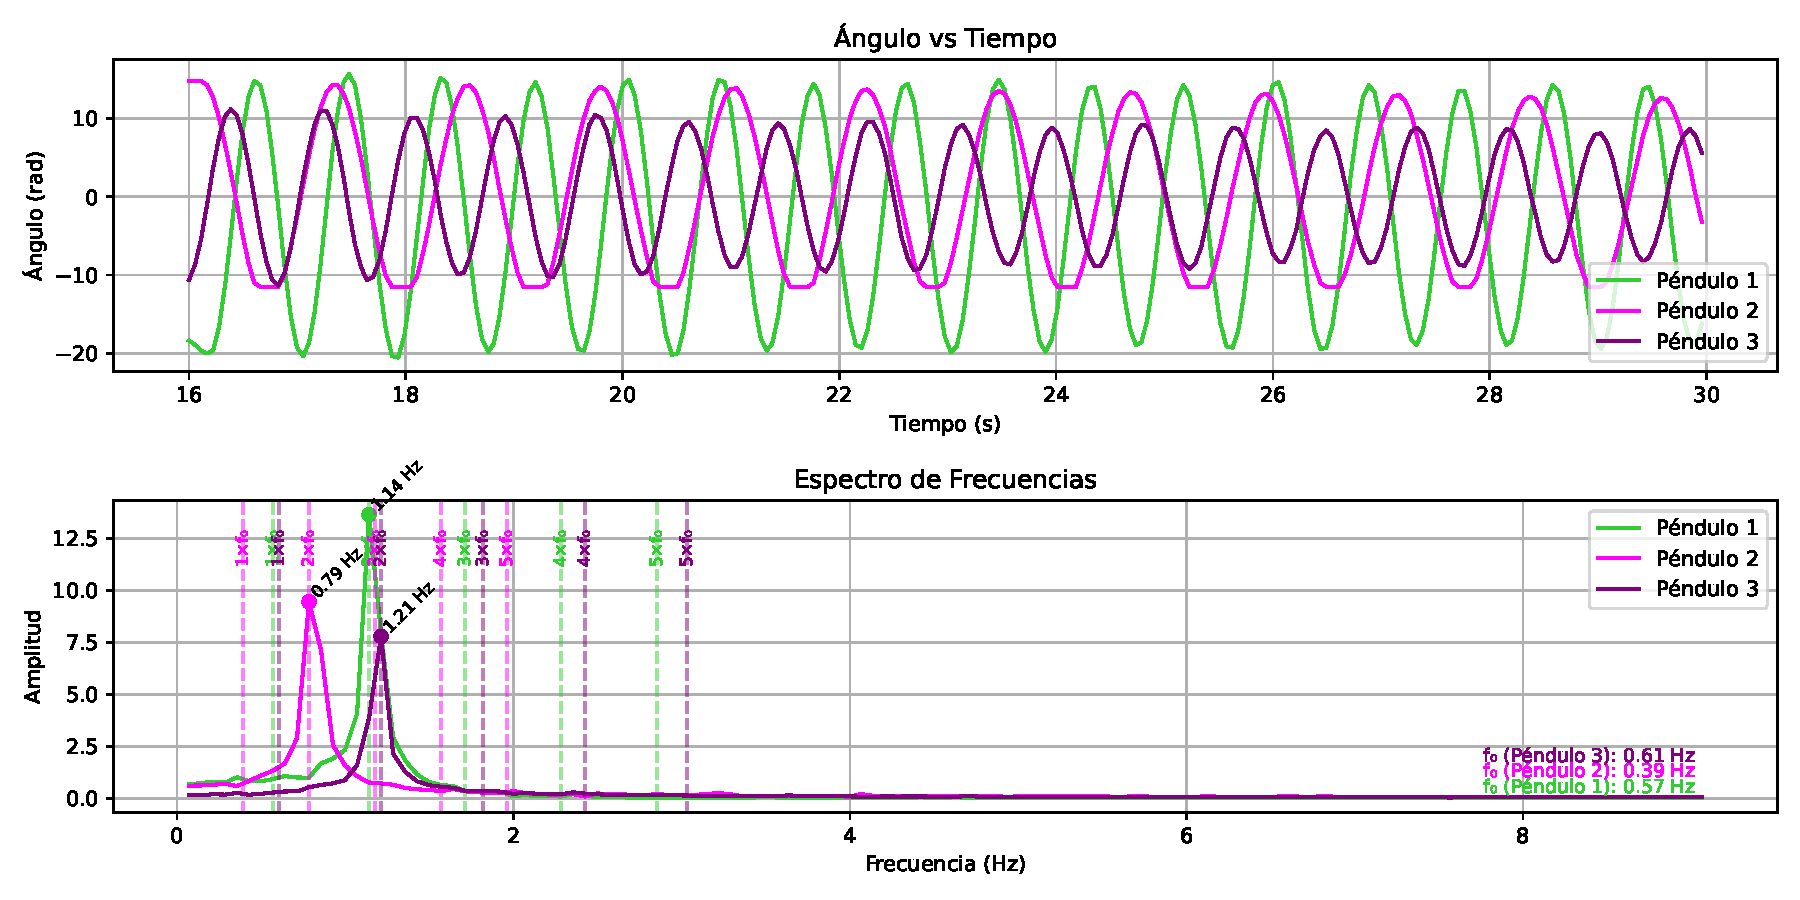
\includegraphics[width=0.8\linewidth]{./Figures/111_11_filtrado.pdf}
  \caption{Evoluci\'on temporal $\theta_i(t)$ y espectro FFT.
  Configuraci\'on 1-1, CI (111).}
  \label{fig:111-11}
\end{figure}

\begin{figure}[htbp!]
  \centering
  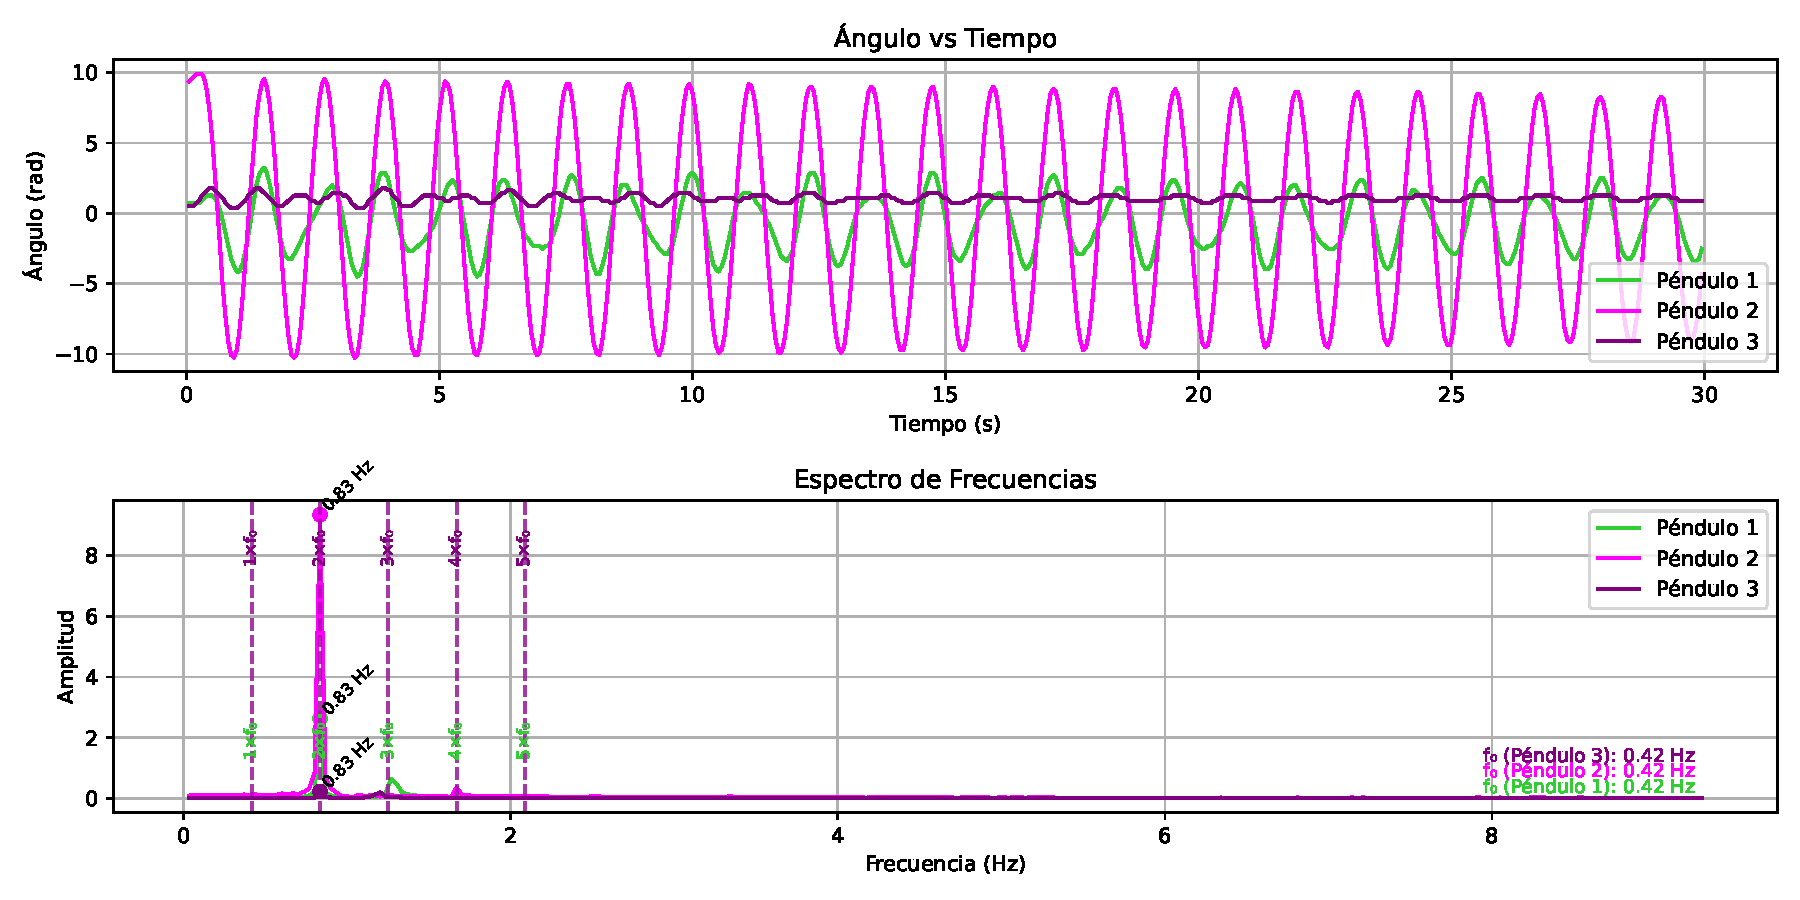
\includegraphics[width=0.8\linewidth]{./Figures/010_15_filtrado.pdf}
  \caption{Evoluci\'on temporal $\theta_i(t)$ y espectro FFT.
  Configuraci\'on 5-1, CI (010).}
  \label{fig:010-51}
\end{figure}

\begin{figure}[htbp!]
    \centering
    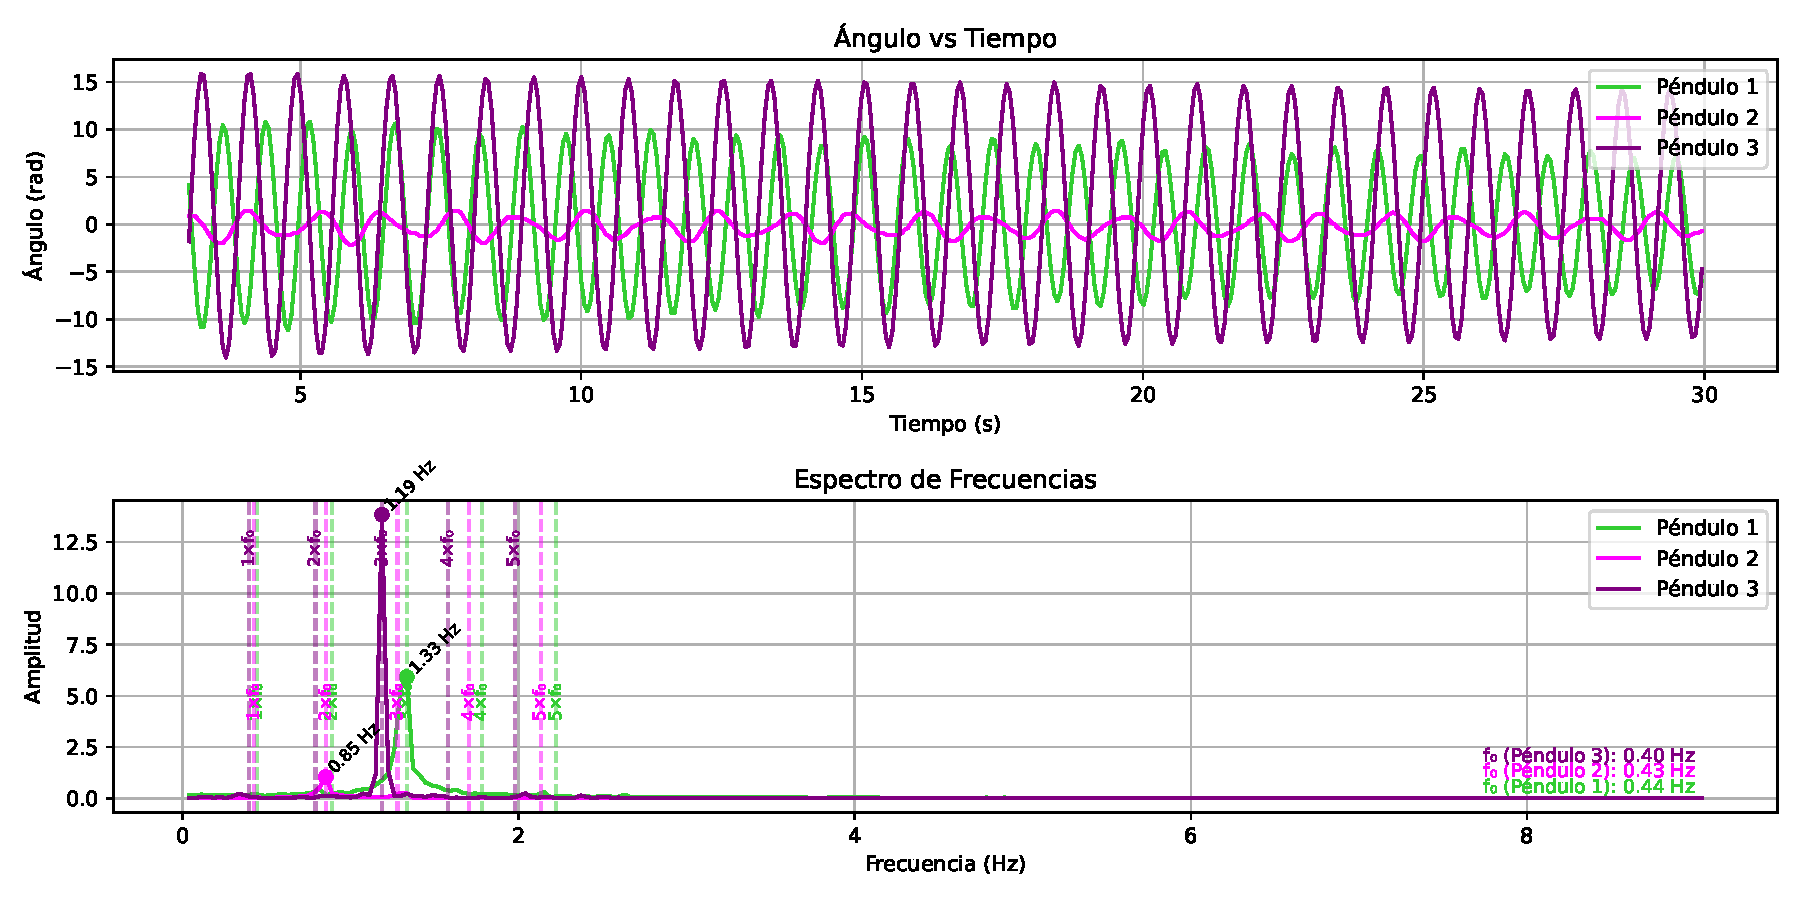
\includegraphics[width=0.8\linewidth]{./Figures/101_16_filtrado.pdf}
    \caption{Evoluci\'on temporal $\theta_i(t)$ y espectro FFT.
        Configuraci\'on 6-1, CI (101).}
    \label{fig:101-61}
\end{figure}

\begin{figure}[htbp!]
    \centering
    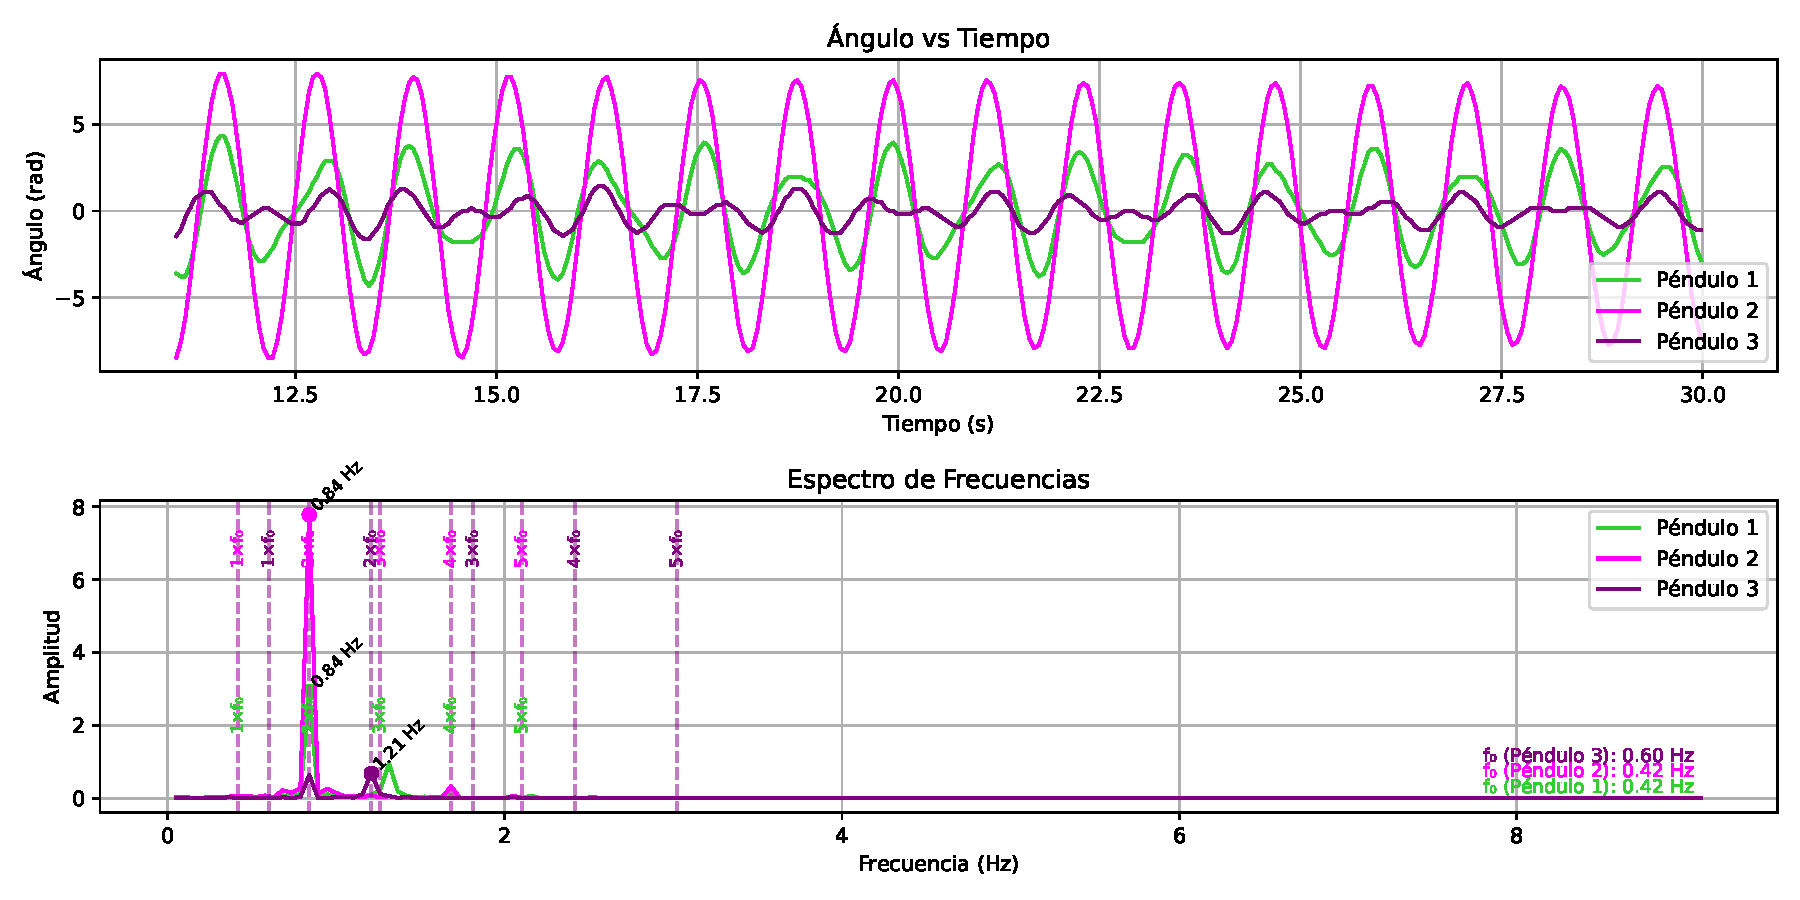
\includegraphics[width=0.8\linewidth]{./Figures/010_26_filtrado.pdf}
    \caption{Evoluci\'on temporal $\theta_i(t)$ y espectro FFT.
        Configuraci\'on 6-2, CI (010).}
    \label{fig:010-62}
\end{figure}

\begin{figure}[htbp!]
    \centering
    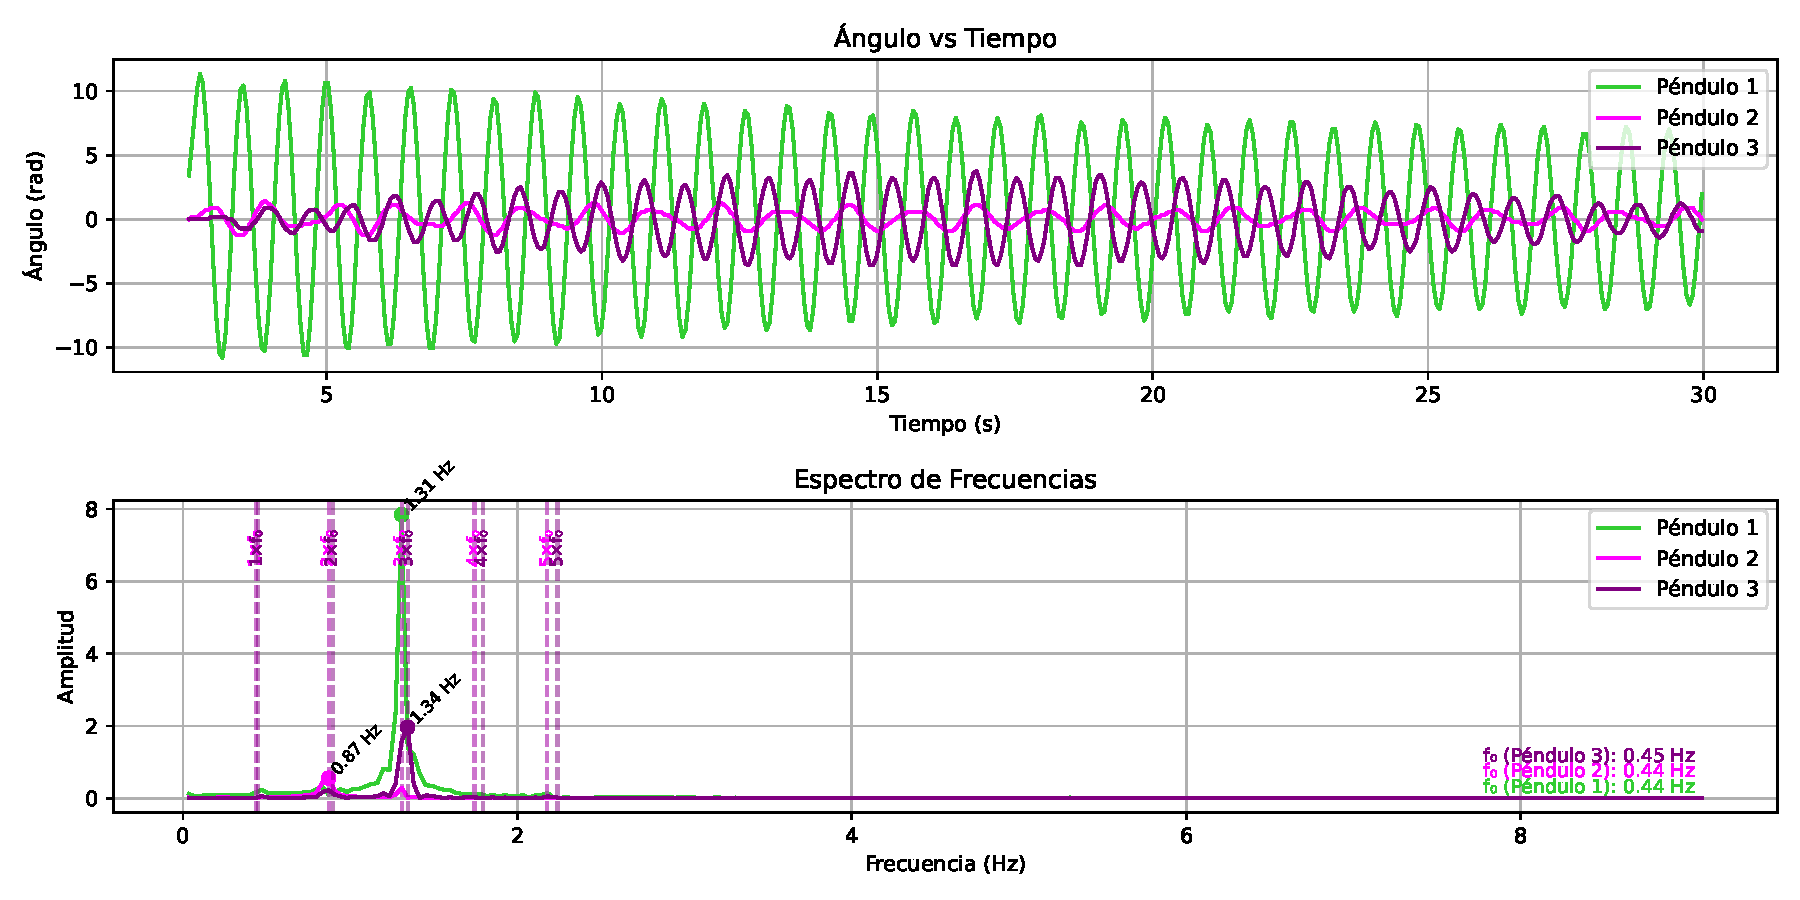
\includegraphics[width=0.8\linewidth]{./Figures/001_66_filtrado.pdf}
    \caption{Evoluci\'on temporal $\theta_i(t)$ y espectro FFT.
        Configuraci\'on 6-6, CI (100).}
    \label{fig:100-66}
\end{figure}

\begin{figure}[htbp!]
    \centering
    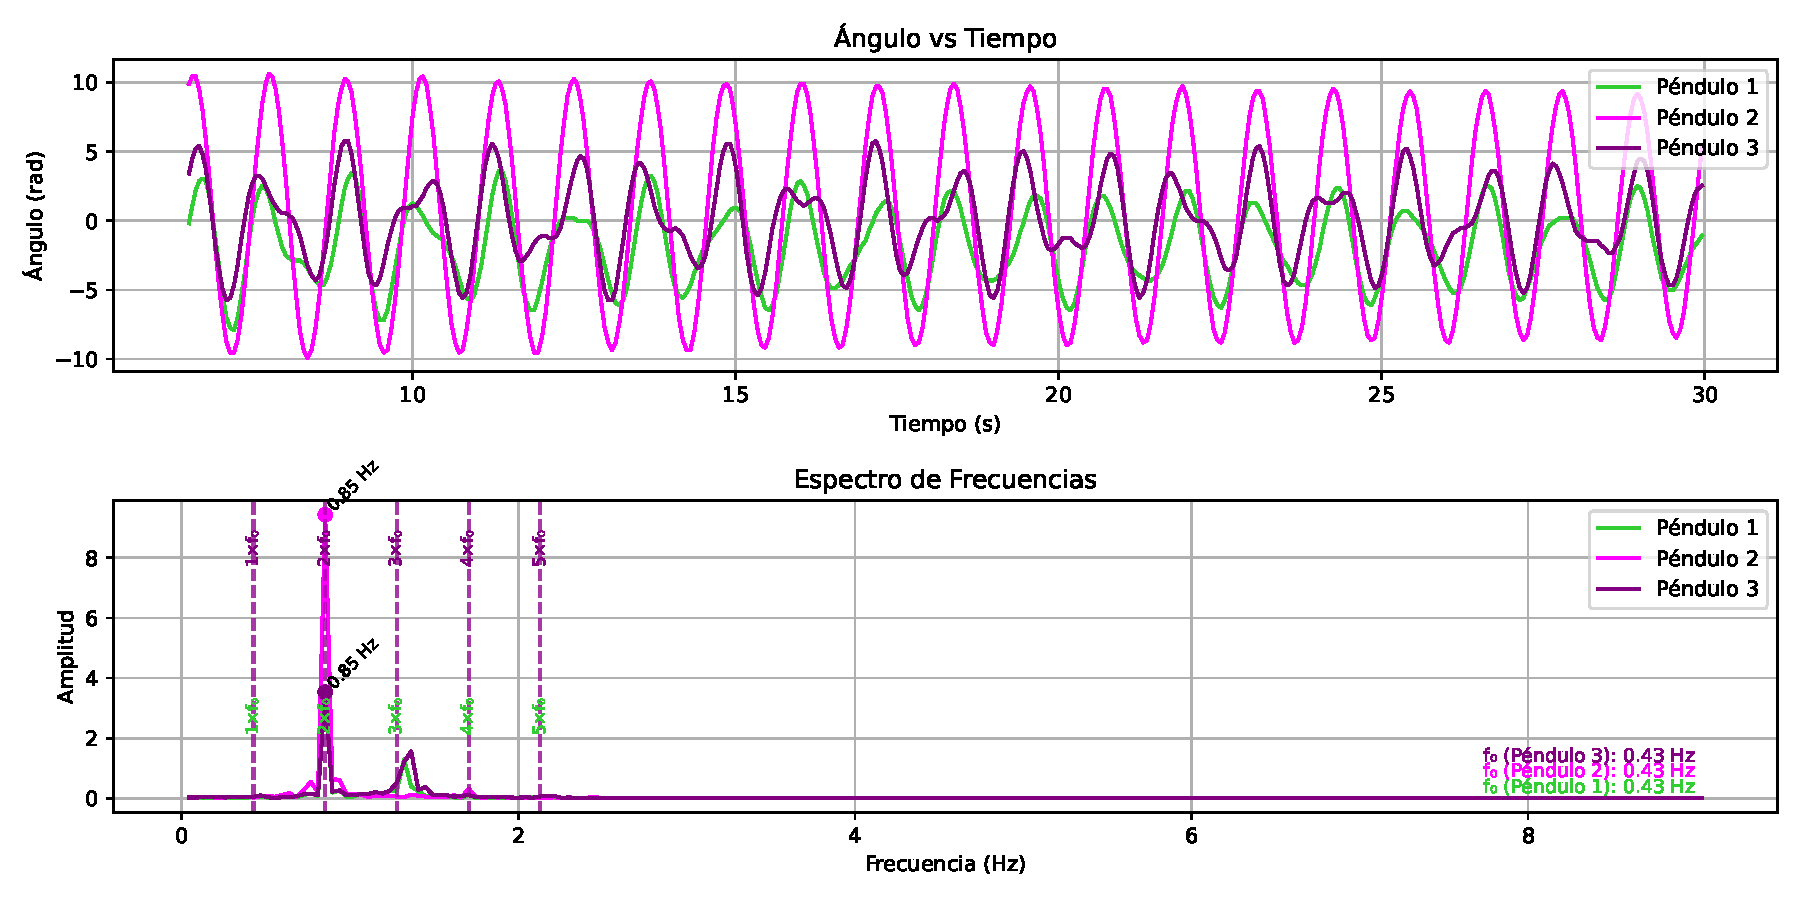
\includegraphics[width=0.8\linewidth]{./Figures/010_66_filtrado.pdf}
    \caption{Evoluci\'on temporal $\theta_i(t)$ y espectro FFT.
        Configuraci\'on 6-6, CI (010).}
    \label{fig:010-66}
\end{figure}

\textbf{An\'alisis de casos espec\'ificos:}

\textbf{\Cref{fig:111-11} (Config. 1-1, CI (111)):}
\begin{itemize}
  \item Cada p\'endulo exhibe un pico de frecuencia principal distintivo en su
    FFT; no comparten una \'unica frecuencia dominante com\'un.
  \item Picos espectrales relativamente anchos: sugiere duraci\'on limitada
    de coherencia o amortiguamiento significativo.
  \item Amortiguamiento esperado: debido a interacciones (acoplamiento,
    fricci\'on) y complejidad del movimiento (laterales desfasados
    respecto al central).
  \item P\'endulo 2: comportamiento temporal con modulaciones en amplitud,
    no arm\'onico simple.
\end{itemize}

\textbf{\Cref{fig:010-51} (Config. 5-1, CI (010)):}
\begin{itemize}
  \item Picos espectrales m\'as definidos y estrechos: comportamiento m\'as
    regular, menos amortiguado para frecuencias dominantes.
  \item Los tres p\'endulos comparten la misma frecuencia principal (reafirma
    tendencia para CI (010)).
  \item Componentes espectrales secundarias comunes, con diferentes
    amplitudes relativas entre p\'endulos.
  \item P\'endulo 3: menor amplitud en componentes espectrales (posiblemente
    menor eficiencia en transmisi\'on de energ\'ia por geometr\'ia de
    acople).
  \item Evoluci\'on temporal m\'as estable y coherente; disminuci\'on gradual
    de amplitudes (amortiguamiento residual).
\end{itemize}

\textbf{\Cref{fig:101-61} (Config. 6-1, CI (101)):}
\begin{itemize}
  \item An\'alisis espectral revela tres picos de frecuencia principales
    distintos (sugiere excitaci\'on de m\'ultiples modos normales).
  \item P\'endulo 3: mayor amplitud en su frecuencia principal y pico
    espectral m\'as estrecho comparado con P1 (relacionado con
    naturaleza del acoplamiento y excitaci\'on inicial de P3).
  \item P\'endulo 2: oscilaciones de amplitud muy reducida (consistente con
    modo normal donde laterales se mueven desfasados y P2 tiene
    participaci\'on m\'inima).
  \item Evoluci\'on temporal: intercambio de energ\'ia entre P1 y P3
    (pulsaciones/batidos), esperado si frecuencias de modos son cercanas
    y hay transferencia de energ\'ia.
\end{itemize}

\textbf{\Cref{fig:010-62} (Config. 6-2, CI (010)):}
\begin{itemize}
  \item P\'endulo 2 (espectro): frecuencia principal con amplitud prominente y
    pico estrecho. Componente secundaria a aprox. $4 f_P$.
    Comportamiento temporal similar a M.A.S.
  \item P\'endulo 1 (espectro): comparte $f_P$ de P2. Otro pico significativo
    a frecuencia $> 3 f_P$. Movimiento no estrictamente M.A.S.,
    pero con clara periodicidad.
  \item P\'endulo 3 (espectro): dos picos con amplitudes comparables,
    frecuencias corresponden aprox. con valores te\'oricos esperados
    (\qty{0.83}{\Hz} y \qty{1.2}{\Hz}). Amplitudes bajas, oscilaci\'on
    de escasa magnitud.
\end{itemize}

\textbf{\Cref{fig:100-66} (Config. 6-6, CI (100)):}
\begin{itemize}
  \item Geometr\'ia de acople facilita transmisi\'on efectiva de energ\'ia.
  \item An\'alisis espectral: los tres p\'endulos comparten componentes de
    frecuencia en mismas ubicaciones espectrales.
  \item P1 y P3 comparten frecuencia principal com\'un (m\'as alta).
  \item P2 tiene su propia $f_P$ (menor), pero exhibe picos secundarios en
    frecuencias donde P1 y P3 oscilan predominantemente (participa en
    modos de mayor frecuencia).
  \item Comportamiento (todos oscilan significativamente) distingue esta
    combinaci\'on, resaltando papel determinante de posici\'on de acoples.
\end{itemize}


\printbibliography

\end{document}
